\chapter{Digital Authentication}
\label{cha:pki}

% \suebox{Digital authentication using PKI is well suited for
%   authentication in distributed environments such as the internet.  We
%   present some of the details here, and how they are expressible in the
%   logic.} \vspace*{1em}

% \section{Digitally Signed Statements and Authority}
% \label{sec:digital-signatures}

%\subsection{Authentication}
%\chapter{Digital Authentication}

To make reasoned access-control decisions in a digital world, we need
to explore in more depth how statements are signed and authenticated
digitally.  The basis for digital signatures rests on cryptographic
keys and cryptographic hash functions in general, and on public-key
cryptography in particular. Digital authentication using
\mainindex{PKI|see{public-key infrastructure}}public-key infrastructure
(PKI) is well suited for authentication in distributed environments
such as the Internet.

In this chapter, we describe the details of digital authentication using
the access-control calculus.  Unlike traditional explanations, we do not
go into the algorithmic details of any particular encryption or hash
function. Rather, we describe the relationship between public and
private keys, encryption and decryption, keys and principals, and
certificates.

% In addition to the discussion on digital signatures, we also develop the
% concept of recognizing authority, which we call \emph{jurisdiction}.  As
% we will see later on in this section, acquiring a belief in a statement
% or cryptographic key usually requires two components: first, a statement
% attributable to some authority, and second, jurisdiction and trust in
% the integrity of the authority making the statement.

\section{Public-Key Cryptography}
\label{sec:pubkey-crypto}


\mainindex{cryptography!public-key cryptography}At the core of
public-key cryptography are two cryptographic keys: one is
\mainindex{public-key infrastructure!public key}\emph{public} and is
openly shared (much like a telephone number or email address), and the
other is \mainindex{public-key infrastructure!private
  key}\emph{private} and must be known \emph{only} by a single
principal. In theory, the principal who possesses the private key is
the only principal who can decrypt messages that were encrypted using
the corresponding public key.  This property is used to ensure
\mainindex{privacy}\emph{privacy}: that is, only a principal with the
correct private key can read a message. Similarly, messages encrypted
using a private key can be universally decrypted by anyone who
possesses the corresponding (and publicly disclosed) public key.  This
property is used for \mainindex{authenticity}\emph{authenticity}: that
is, one can establish the identity of the author of a message.

The public key $K$ and private key $K^{-1}$ together form a
\mainindex{public-key infrastructure!key pair}\emph{key pair}
$(K,K^{-1})$, and each key can undo the actions of the other.  That
is, if \emph{encrypt} and \emph{decrypt} are particular encryption and
decryption functions, then the following properties must hold for all
messages $m$:
\begin{eqnarray*}
  \mathit{decrypt}(K^{-1},\mathit{encrypt}(K,m)) & = & m, \\
  \mathit{decrypt}(K, \mathit{encrypt}(K^{-1},m)) & = & m. 
\end{eqnarray*}
In addition, the public and private keys are typically distinct (i.e.,
$K^{-1} \neq K$).  Consequently, public-key cryptography is often
referred to synonymously as \mainindex{asymmetric-key
  cryptography}\emph{asymmetric-key cryptography}.  In the case of
public-key algorithms such as RSA \cite{RSA}, the same algorithm
serves both to encrypt and decrypt messages.

\mainindex{cryptography!cryptosystem, key properties of}There are two additional
properties about encryption and decryption that are important if a
cryptosystem is to be useful:
\begin{enumerate}
\item It should be computationally infeasible to read an
  encrypted message without knowing the correct decryption key.  

  That is, given an encrypted message $\mathit{encrypt}(K_e,m)$, it
  should be computationally infeasible to determine $m$ without knowing
  the reciprocal key $K_d$.  (Note that $K_e$ may be either a public or
  private key; $K_d$ is the other half of the key pair.)
\item It should be computationally infeasible to successfully forge an
  encryption without knowing the encryption key $K_e$.

  That is, given a message $m$ but without knowing $K_e$, it should be
  computationally infeasible 
  to compute an $\mathit{x}$ such that $\mathit{decrypt}(K_d,x) = m$.  
\end{enumerate}

\mainindex{privacy!use of cryptography for}These properties of
public-key cryptography support privacy in the following way.  If
Alice wishes to send a message to Bob that only Bob can read, she
encrypts the message with Bob's \emph{public key} $K_{\name{Bob}}$.
Thus, Alice sends to Bob the following:
\[ \mathit{encrypt}(K_{\name{Bob}},\mathrm{message}). \]
The idea here is that the resulting cipher text should
be decipherable only with knowledge of Bob's \emph{private key}
$K_{\name{Bob}}^{-1}$.  Upon receipt, Bob uses his private key to
decrypt the message:
\[
\mathit{decrypt}(K^{-1}_{Bob},\mathit{encrypt}(K_{\name{Bob}},\mathrm{message})). \] 
Figure~\ref{fig:public key} illustrates schematically how Alice and Bob
use Bob's keys to ensure privacy of the message sent to Bob.

% More
% precisely, if $K_{\name{Bob}}$ is Bob's public key available to all, and
% $K^{-1}_{Bob}$ is Bob's private key known only to Bob:
% \begin{eqnarray*}
%   \textsf{Private message sent to Bob} & = & \mathit{encrypt}(K_{\name{Bob}},\mathrm{message})\\
%   \textsf{Deciphered message} & = & \mathit{decrypt}(K^{-1}_{Bob},\mathit{encrypt}(K_{\name{Bob}},\mathrm{message}))
% \end{eqnarray*}

\begin{figure}[tbp]
  \centering
  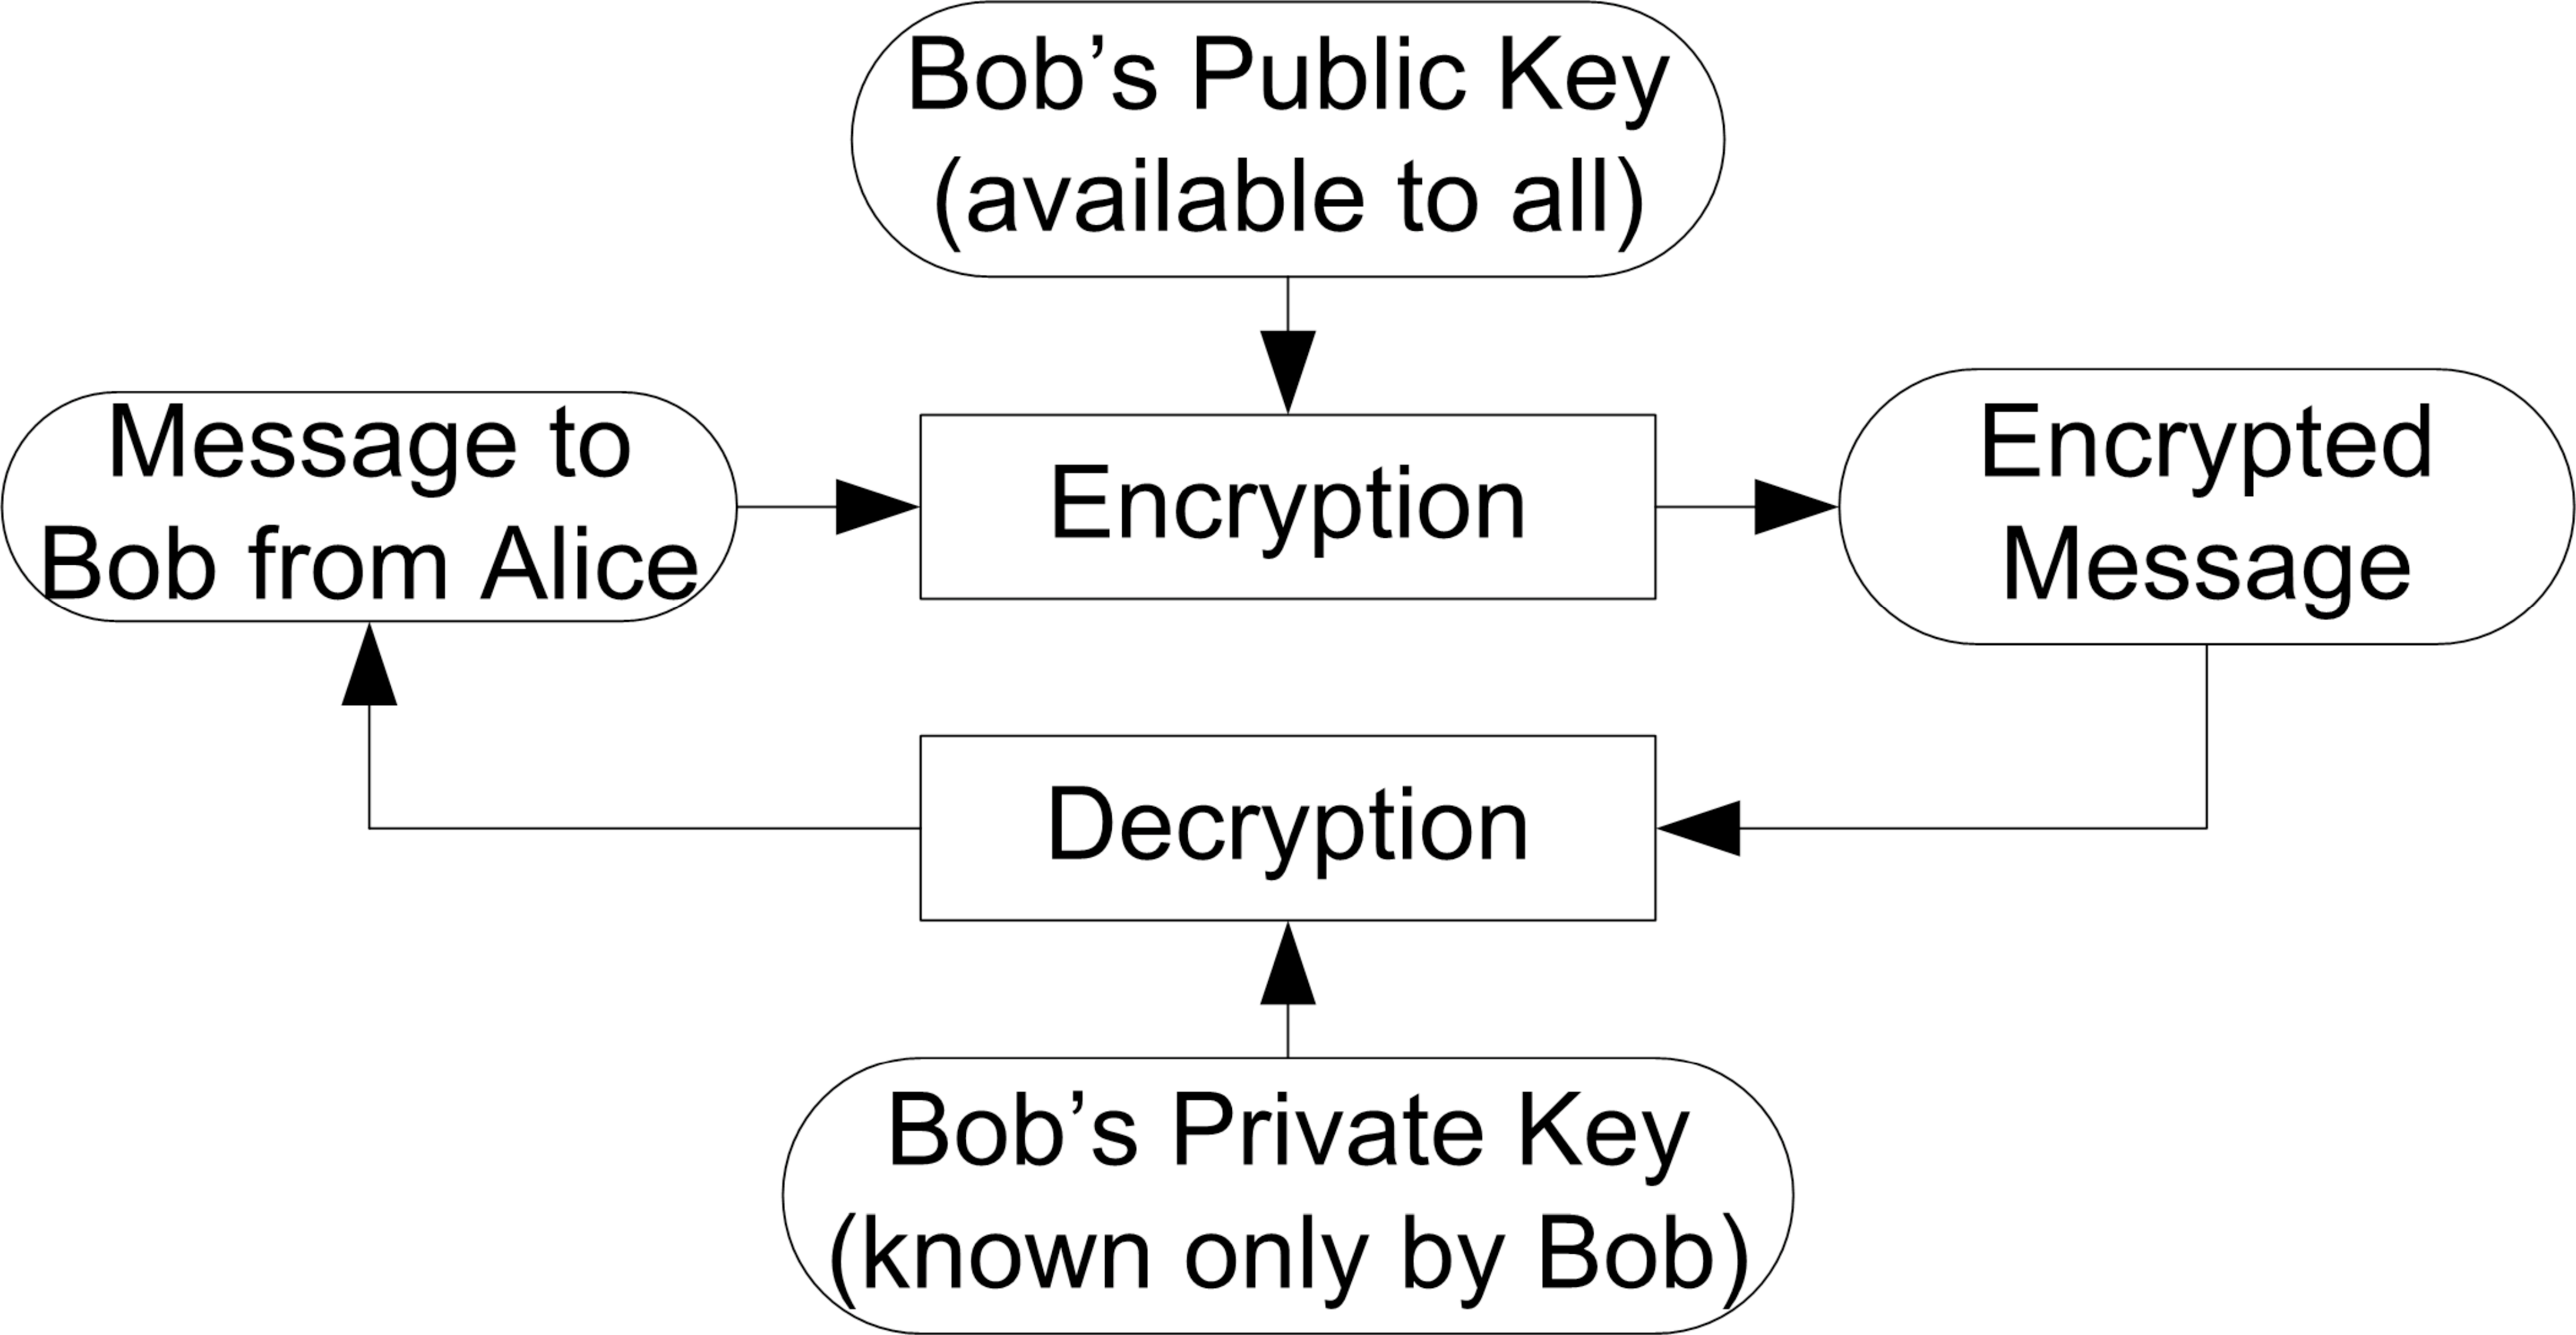
\includegraphics[width=3.5in]{Figures/pki/publicKey}
  \caption{Process for using public-key encryption for privacy}
  \label{fig:public key}
\end{figure}


The use of public-key cryptography is not limited solely to achieving
privacy. More often, it is used to authenticate messages, such as
website-connection requests, public-key certificates, and so on.  For
example, suppose that Bob wishes to communicate a message to the world
in such a way that anyone can deduce that Bob authored the message. Such
a situation might arise if Bob needs to establish his authorship of an
article or book for intellectual-property protection.  In this case, Bob
can encrypt his book using his \emph{private key} (which is known only
by him):
\[ \mathit{encrypt}(K^{-1}_{\name{Bob}}, book). \]
Anyone who cares to read
Bob's book can read it using Bob's freely available \emph{public
  key} to decrypt his encrypted file:
\[ \mathit{decrypt}(K_{\name{Bob}},\mathit{encrypt}(K^{-1}_{Bob},
book)). \] The idea here is that \emph{only} Bob could have created the
original encrypted file, because only Bob knows the key
$K^{-1}_{\name{Bob}}$ used to create it.  This sort of use of public-key
  cryptography for authenticity is illustrated in
  Figure~\ref{fig:private key}.
% \begin{eqnarray*}
%   \textsf{Book authored by Bob} & = & \mathit{encrypt}(K^{-1}_{Bob}, book)\\
%   \textsf{Book accessible by Bob's public key} & = & \mathit{decrypt}(K_{\name{Bob}},\mathit{encrypt}(K^{-1}_{Bob}, book))
% \end{eqnarray*}

\begin{figure}[tbp]
  \centering
  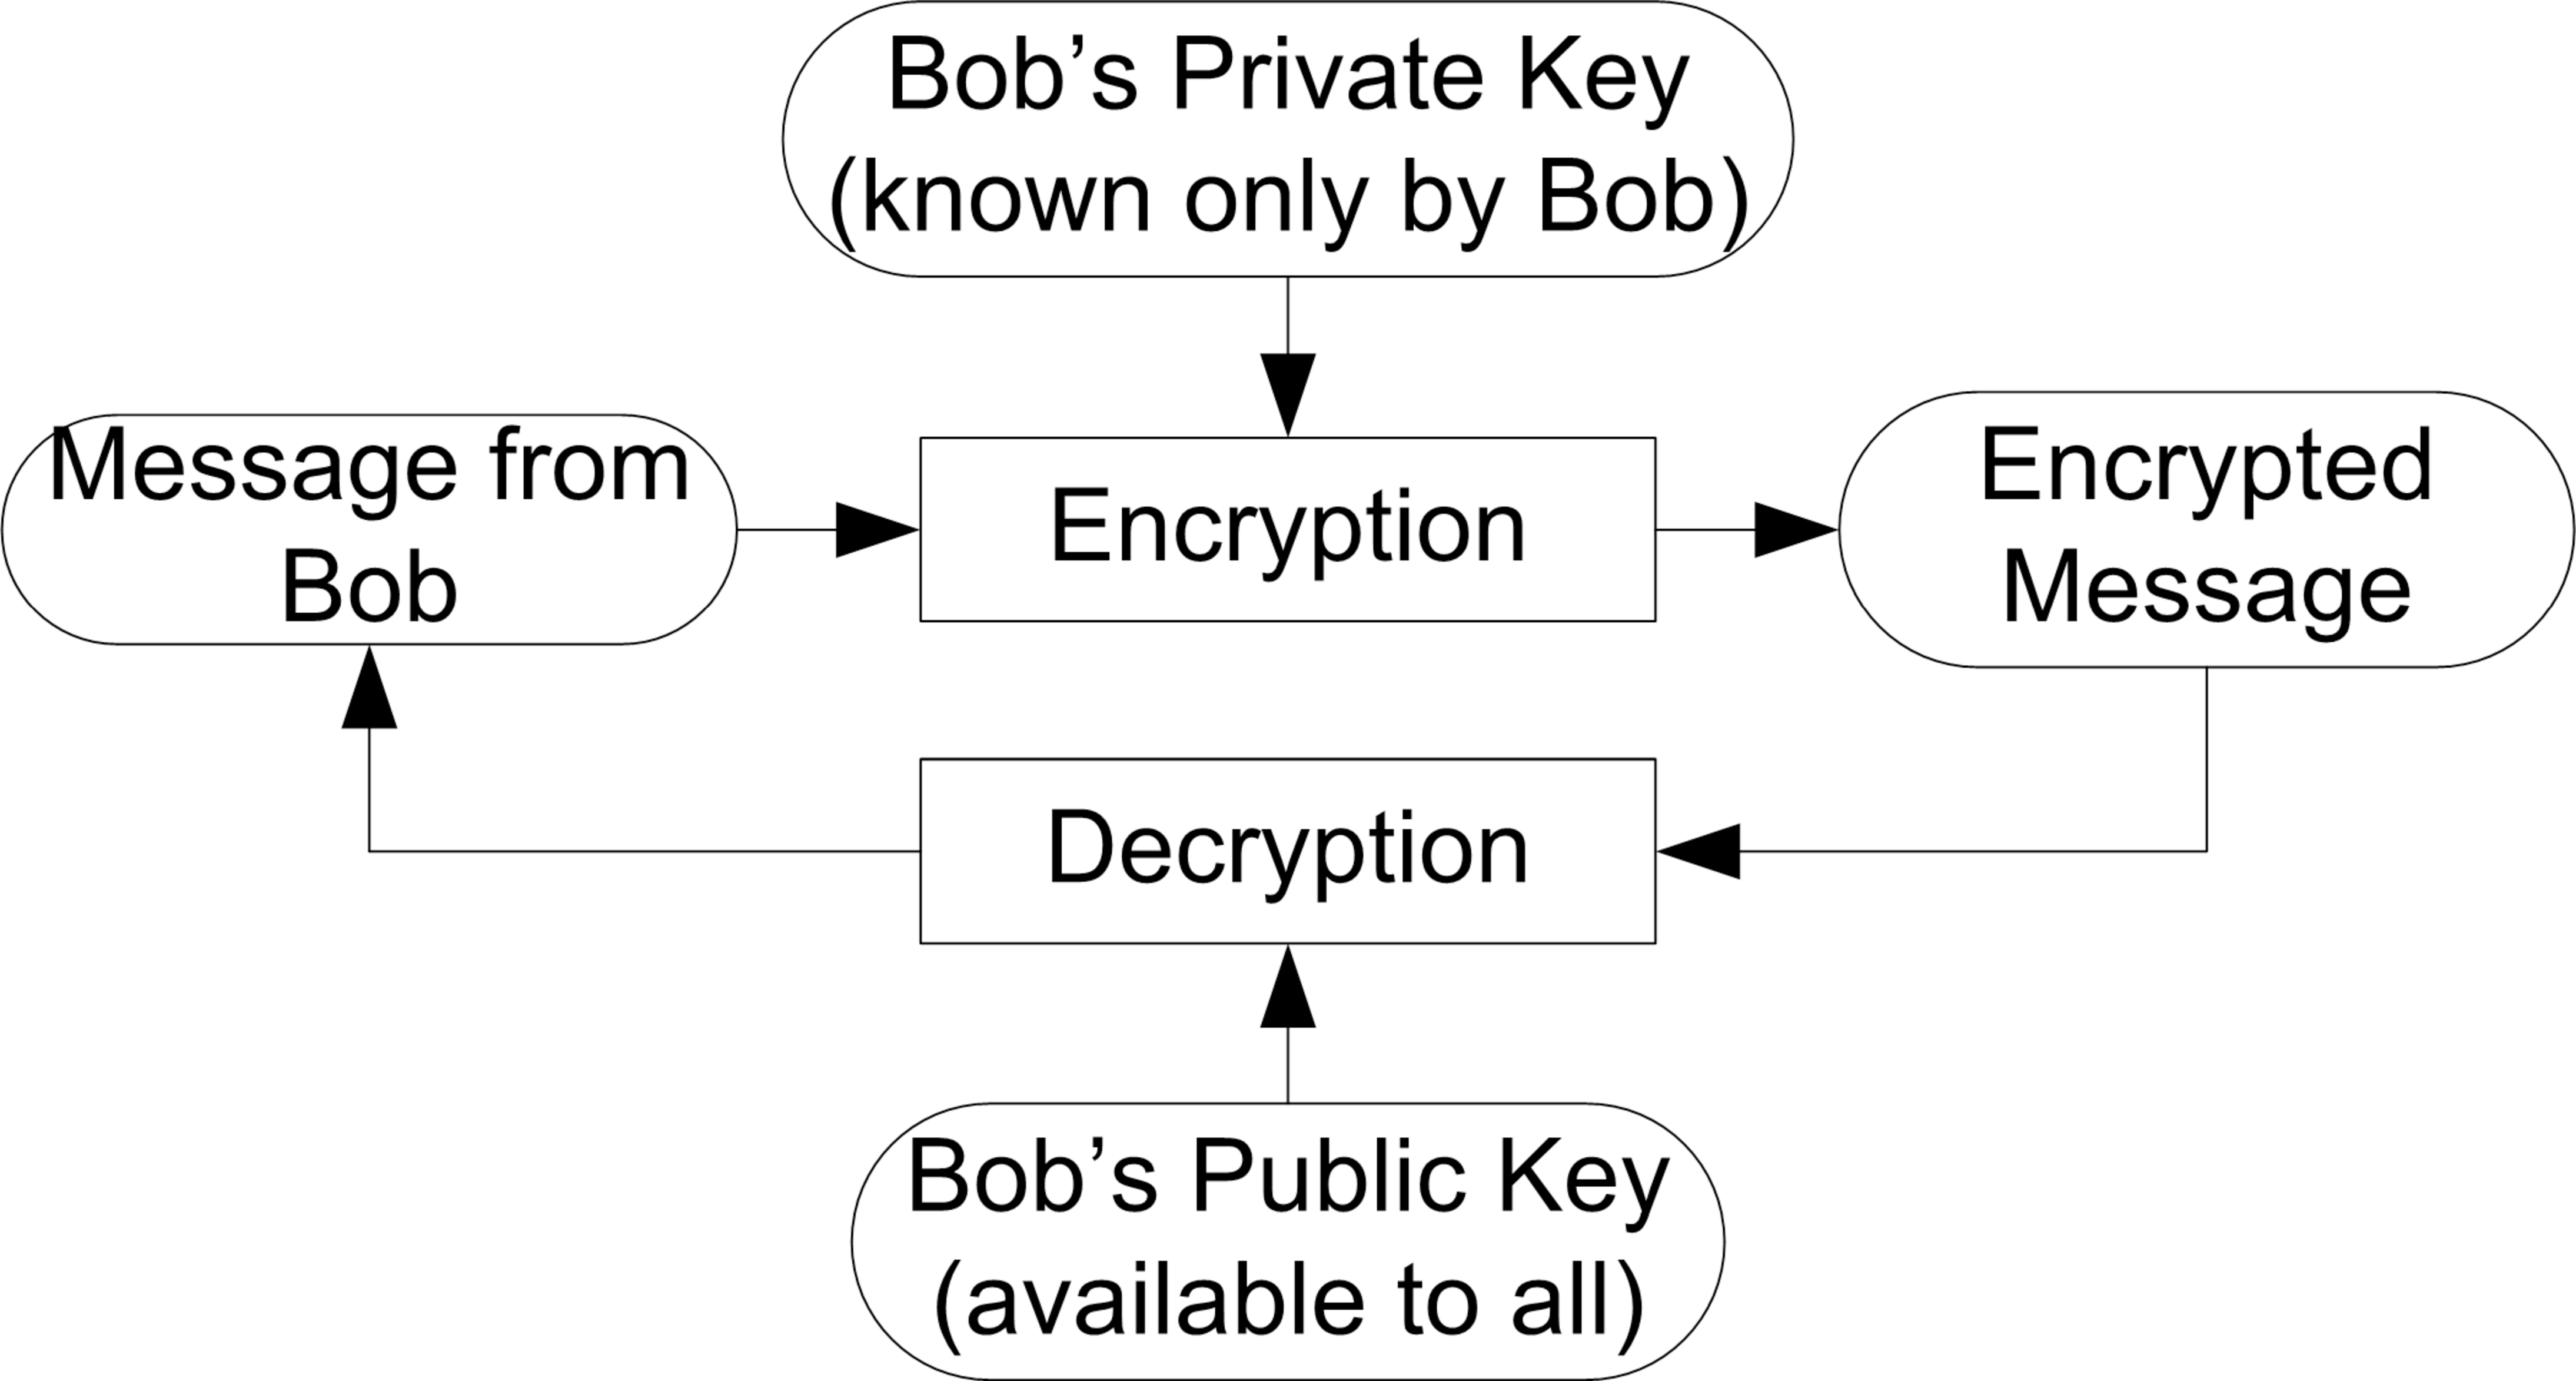
\includegraphics[width=3.5in]{Figures/pki/privateKey}
  \caption{Process for using private-key encryption for authenticity}
  \label{fig:private key}
\end{figure}

\mainindex{authenticity!use of cryptography for}One can combine these
two approaches to achieve a combination of \mainindex{privacy}privacy
and \mainindex{authenticity}authenticity.  For example, suppose that
Alice wants to send a message that only Bob can read, while providing
Bob assurance that the message is coming from her.  To achieve this
goal, Alice employs the following three-step process:
\begin{enumerate}
\item Alice encrypts her message $m$ with her \emph{private key}:
  \[ \mathit{encrypt}(K^{-1}_{\name{Alice}},m). \] This step will allow
  Bob to deduce that Alice authored the message $m$, because Bob can
  retrieve $m$ using Alice's \emph{public key}.
\item Alice encrypts the result from step one with Bob's \emph{public
    key}, resulting in the following:
  \[
  \mathit{encrypt}(K_{\name{Bob}},\mathit{encrypt}(K^{-1}_{\name{Alice}},m)).
  \]
  This step provides Alice with assurance that only Bob can read her
  message, because only Bob's private key will be able to decrypt this
  cipher text.
\item Alice informs Bob in plain text that she is the author of the
  cipher text from step two.  This hint tells Bob to look up Alice's
  public key so that he can decipher the message in such a way as to be
  assured that Alice was the author.  
\end{enumerate}

\section{Efficiency Mechanisms}
\label{sec:digital-signatures}
In theory, the approaches described in the previous section are
sufficient to handle the needs of privacy and authenticity. In practice,
however, the approaches described for authenticity are rarely used,
because public-key algorithms are relatively slow and costly to use.  In
addition, the repeated use of a given key-pair on large amounts of text
can expose the keys and make them vulnerable to cryptographic analysis
and discovery. To address these pragmatic concerns, two additional steps
can be taken: (1) we can use a \emph{cryptographic hashing} algorithm,
and (2) we can use a \emph{session} or \emph{data-encryption key}
(DEK). We describe these steps---and their use in creating and verifying
digital signatures---in this section.

\subsection{Cryptographic Hash Functions}

% \begin{figure}[tbp]
%   \centering
%   \includegraphics{Figures/basicACConcepts/hash}
%   \caption{Hash functions}
%   \label{fig:hash functions}
% \end{figure}

% Cryptographic hash functions take arbitrarily large files and return a
% fixed-length number (e.g., 128-bits). % This is shown in
% % Figure~\ref{fig:hash functions}. 

% Hash functions are widely used, but not all are cryptographic in nature.
% An odd parity bit that is set when there is an odd number of $1$'s
% stored in a memory location is a hash function that is not cryptographic
% in nature.  For example, consider an odd parity bit for 4-bit words.
% The 4-bit words that would set the parity bit to a $1$ are as follows:
% $0001$, $0010$, $0100$, $1000$, $0111$, $1011$, $1101$, $1101$, and
% $1110$.  The predictability of the odd parity bit function disqualifies
% it as a cryptographic hash.  If the parity bit is $1$, then the input is
% one of the nine 4-bit numbers above.  If the parity bit is $0$, then it
% is one of the remaining seven 4-bit numbers that have an even number of
% $1$'s or all $0$'s.

Hash functions are commonly used in computing as a way to map large data
spaces to more compact spaces, substituting uniqueness for efficiency.
A very simple example of a hash function is a word-level \emph{parity
  check}: all $32$-bit words with an even number of $1$ bits are mapped
to the bit $0$, while all those with an odd number of $1$ bits are
mapped to the bit $1$.  In this case, a data space with $2^{32}$
elements is mapped to a data space of $2$ elements, at the cost of
uniqueness: $2^{16}$ values are hashed to the bit $0$, and $2^{16}$
values are hashed to the bit $1$.

\mainindex{hash function, cryptographic}\emph{Cryptographic hash
  functions} are hash functions with an additional property: given any
particular hash value, it must be \emph{computationally infeasible} to
determine an input that, when hashed, produces the given value.  This
property is known as the \mainindex{hash function,
  cryptographic!one-way property}\emph{one-way property} of
cryptographic hashes: while hash values can be computed easily from a
given input, it is computationally infeasible to do the reverse (i.e.,
compute an input that produces a particular hash value).  Thus, for
example, the parity check clearly fails the one-way property (and
hence would not make for a cryptographic hash function), because it is
trivial to find 32-bit words with parity $1$.

The one-way property of cryptographic hashes makes it possible for
fixed-length cryptographic hash values to simulate unique identifiers
for messages of arbitrary length.  For example, suppose Ellen wants to
send a file to Todd that is several megabytes in length, and she wants
Todd to be able to determine whether the file he receives has arrived
unchanged and uncorrupted.  To accomplish this goal, Ellen sends a
\mainindex{hash function, cryptographic}\emph{cryptographic hash} of
the file---also known as the \mainindex{hash function,
  cryptographic!checksum}\emph{cryptographic checksum}---along with
the file itself:
\[ (\mathit{file}, \textit{cryptographic checksum}).\] When Todd receives
the file and the cryptographic checksum, he applies the hash algorithm
to the received file and compares the value he computed with the
checksum sent by Ellen.  If they both match, then Todd concludes that the
file he received is intact and free of any tampering or corruption.


\subsection{Data-Encryption Keys}
When privacy is also a concern for a large file, the sender may elect
to also employ a \mainindex{symmetric key}\emph{symmetric-key}
encryption algorithm---such as the Advanced Encryption Standard (AES)
\cite{AES}---to create a one-time \mainindex{data-encryption
  key}data-encryption key $K_{dek}$.  Symmetric-key encryption
algorithms use the same key for both encryption and decryption (i.e.,
$K_{dek} = K^{-1}_{dek}$).  In addition, symmetric-key encryption
algorithms are three orders of magnitude faster than typical
public-key algorithms, because of the underlying operations they
employ (i.e., exclusive-or and bit substitutions as opposed to
modulo-$n$ exponentiation).

% If privacy is a concern as well as not overusing public keys on large
% files, what Ellen can do is create a one-time data-encryption key
% $K_{dek}$ for a \emph{symmetric} key encryption algorithm such as the
% Advanced Encryption Standard (AES) \cite{AES}.  Symmetric key encryption
% algorithms are called symmetric because the same key is used for both
% encryption and decryption. In other words, $K_{dek} = K^{-1}_{dek}$.

If Ellen chooses this approach, she first creates a key $K_{dek}$; she
then encrypts the file with $K_{dek}$, computes the cryptographic
checksum of the file, and encrypts $K_{dek}$ with Todd's public key
$K_{\name{Todd}}$. Ellen sends these three items to Todd:
\[ \mathit{encrypt}(K_{\name{Todd}},K_{dek}), \qquad
\mathit{hash}(\mathit{file}), \qquad \mathit{encrypt}(K_{dek},
\mathit{file}). 
\]
% \begin{eqnarray*}
%   \textsf{Data Encryption Key encrypted for Todd} & = & \mathit{encrypt}(K_{\name{Todd}},
%   K_{dek}) \\
%   \textsf{File encrypted with }K_{dek} & = & \mathit{encrypt}(K_{dek}, file)\\
%   \textsf{Cryptographic Checksum} & = & hash(file)
% \end{eqnarray*}
When Todd receives these three items, he first retrieves the
data-encryption key $K_{dek}$ by using his private key:
\[ \mathit{decrypt}(K^{-1}_{\name{Todd}},\mathit{encrypt}(K_{\name{Todd}},
K_{dek})) = K_{dek}. \]
He then uses the data-encryption key to retrieve the file:
\[ \mathit{decrypt}(K_{dek},\mathit{encrypt}(K_{dek},\mathit{file})) = \mathit{file}.\]
Finally, he checks the integrity of the retrieved file by determining
whether it hashes to the cryptographic checksum that Ellen sent.  

Unfortunately, however, this scheme is subject to fraud, because none of
the sent items directly tie Ellen to the message that Todd receives.  As
a result, a third party could send their own message (along with its
cryptographic checksum) to Todd, alleging that the message is from
Ellen. Todd has no way of determining the truth of such a claim.  We
can address this problem by introducing digital signatures in the
next subsection.

\subsection{Digital Signatures}

\begin{figure}[tbp]
  \centering
  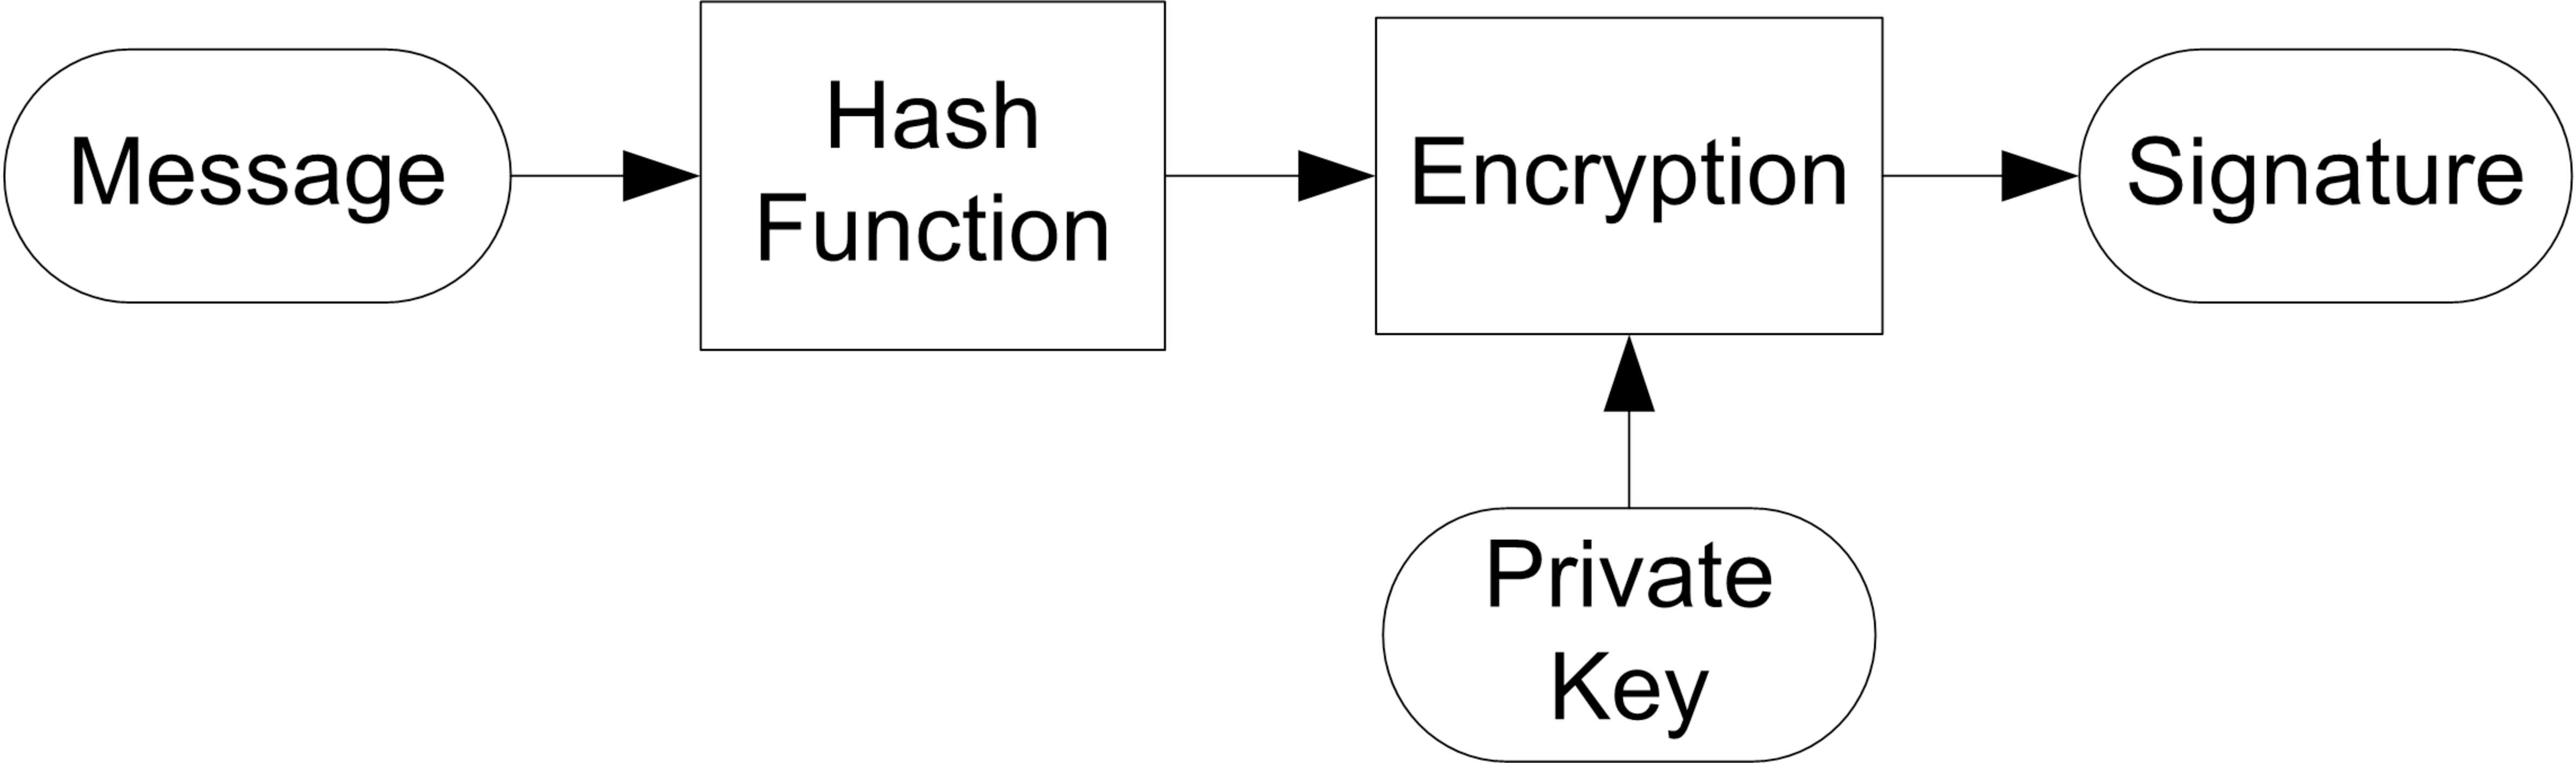
\includegraphics[width=3.5in]{Figures/pki/signature}
  \caption{Process for creating a digital signature}
  \mainindex{digital signature}
  \label{fig:digital signature}
\end{figure}

We can fix the potential fraud problem by one addition: Ellen creates
a \mainindex{digital signature}\emph{digital signature} by encrypting
the cryptographic checksum with her \emph{private key}.
Figure~\ref{fig:digital signature} illustrates a process for creating
digital signatures that supports both integrity and authorship:
\begin{enumerate}
\item The message or file is hashed by a one-way function. The resulting
  fixed-length hash value identifies the contents of the message.
\item The hash value is then encrypted using the \emph{private} key of
  the sender. The encrypted hash value identifies the sender, because
  the hash value can be retrieved only by using the sender's public
  key.  Note that, because the hash value is much smaller than the
  message itself, this approach is much more efficient than the process
  described in Section~\ref{sec:pubkey-crypto}.
\end{enumerate}
Unlike human signatures, which remain relatively unchanged over time,
digital signatures change depending on the contents of what is being
signed.

\begin{figure}[tbp]
  \centering
  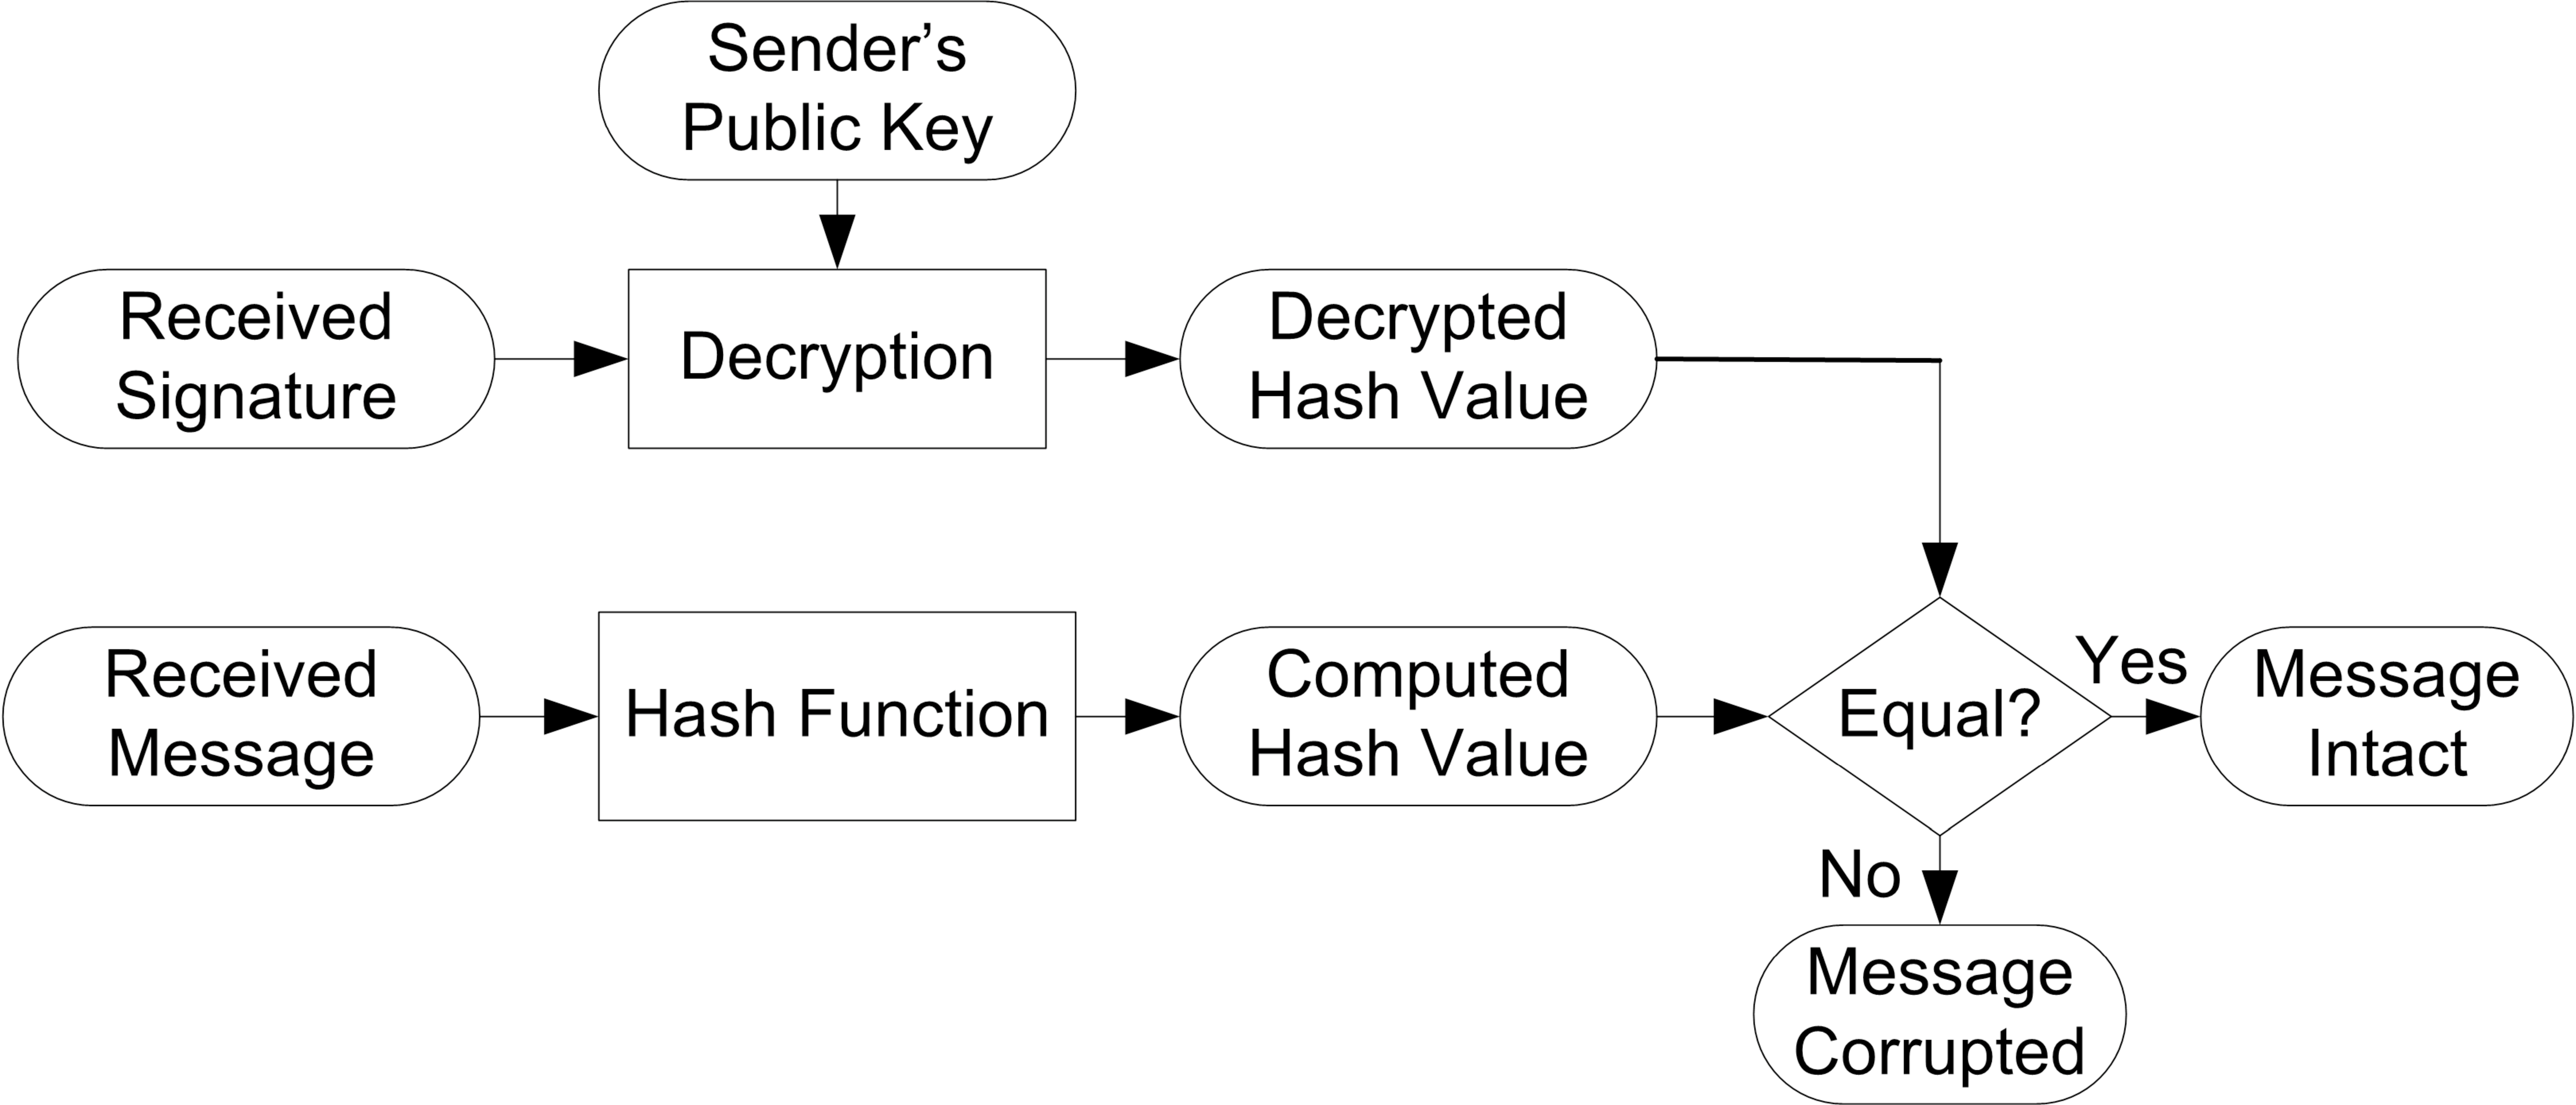
\includegraphics[width=4.5in]{Figures/pki/signatureCheck}
  \caption{Process for verifying a digital signature}
  \mainindex{digital signature}
  \label{fig:signature verification}
\end{figure}

\mainindex{digital signature}Figure~\ref{fig:signature verification}
illustrates the process of verifying a digital signature.  The process
simply compares the following two values: (1) the hash value obtained
by decrypting the received signature using the sender's public key,
and (2) the hash value obtained by hashing the contents of the
received message.  If the values match, then the received message is
considered to be both intact and from the public key's owner.



\section{Reasoning about Cryptographic Communications}
In the previous two sections, we have seen how cryptography can be used
to provide assurances of privacy and authenticity in distributed digital
systems.  In this section, we see how the access-control logic can be
used to express and reason about cryptographic communications.

As an example, suppose that Ellen uses the methods described in
Section~\ref{sec:digital-signatures} to send Todd a digitally signed
message.  For this first case, let us imagine that Ellen sends the
message itself in the clear (i.e., in plaintext with no encryption), but
she digitally signs it.  Thus, she sends to Todd the following
combination of items:
\[ m,\quad \mathit{encrypt}(K^{-1}_{\name{Ellen}},hash(m)).\]
That is, she sends the message $m$, along with the encrypted hash (i.e.,
cryptographic checksum) of $m$. 

When Todd receives the message, he applies the \mainindex{authentication!message
  integrity, formalization in logic} signature-verification protocol
of Figure~\ref{fig:signature verification}.  If this process is
successful, then Todd has evidence that Ellen's public key
$K_{\name{Ellen}}$ has been used to verify that the message $m$
arrived intact and uncorrupted.  This fact can be expressed in the
access-control logic by recognizing $m$ as a statement made by
$K_{\name{Ellen}}$:
\[ K_{\name{Ellen}} \says m .\]
If Todd believes that  $K_{\name{Ellen}}$ is Ellen's public key---perhaps
he looked her key up in a public directory, or perhaps Ellen gave it to
him sometime in the past---then he is willing to associate statements
made (i.e., integrity-checked) by that key with Ellen.  Thus, the belief
that Ellen's public key is $K_{\name{Ellen}}$ can be expressed in the
logic as the following statement:
\[ K_{\name{Ellen}} \speaksfor \name{Ellen} . \] Based on these two
factors, Todd can deduce that Ellen originally sent the message $m$.  In
terms of the logic, this analysis uses the \infname{Derived Speaks For}
rule, as shown in the proof of
Figure~\ref{fig:dig-sig-proof}.

\begin{figure}
  \centering
  \begin{formalProof}
    1. $K_{\name{Ellen}} \says m$ & Received message with signature verified
    using $K_{\name{Ellen}}$\\
    2. $K_{\name{Ellen}} \speaksfor Ellen$ & Ellen's public key\\
    3. $Ellen \says m$ & 2, 1 Derived speaks for
  \end{formalProof}
  \caption{Simple analysis of digital signatures}
  \label{fig:dig-sig-proof}
\end{figure}

Having examined the simpler case, now let us consider the case where
Ellen sends Todd a digitally signed message, using a data-encryption key
$K_{dek}$ to encrypt the message.  Recall that Todd receives three items,
along with a hint that Ellen is the sender:
\[ \mathit{encrypt}(K_{\name{Todd}}, K_{dek}), \quad
\mathit{encrypt}(K_{dek},m), \quad
\mathit{encrypt}(K^{-1}_{\name{Ellen}},hash(m)). \]
Todd must decrypt the first component of this package to
obtain the key $K_{dek}$, which he can then use to retrieve the message
$m$.  He then verifies Ellen's digital signature by computing the
cryptographic hash of $m$ and comparing it with the checksum that Ellen
sent.  

If this process is successful, then Todd once again used Ellen's public
key to verify that the message $m$ he received was indeed the one
initially signed by Ellen.  As we saw earlier, this situation can be
expressed simply as follows:
\[ K_{\name{Ellen}} \says m .\]
Although the signature-verification process itself may be more involved
in this situation, it plays the same role in Todd's interpretation of the
received message.  From Todd's perspective, the important aspect is
deducing that the message was initially signed by Ellen using the key
$K^{-1}_{\name{Ellen}}$, which presumably only she possesses. Although
he initially had to decrypt other components of the message using the
keys $K^{-1}_{\name{Todd}}$ and $K_{dek}$, those operations alone do
not associate the message $m$ to Ellen.


% \begin{example}
%   How do we represent this in the access-control calculus? The answer is
%   we represent it as $Ellen \says m$, exactly as it we did in the
%   previous example!  The reason is that from Todd's perspective, what is
%   important is deducing that $m$ as received by Todd was in fact signed
%   by Ellen using $K^{-1}_{\name{Ellen}}$, which presumably only Ellen
%   possesses. While Todd did decrypt both $K_{dek}$ and $m$ using
%   $K^{-1}_{\name{Todd}}$ and $K_{dek}$ respectively, these operations themselves
%   do not contribute anything to an argument attributing $m$ to Ellen.
%   Of significance was verifying the signature using $K_{\name{Ellen}}$ and
%   knowing that $K_{\name{Ellen}} \speaksfor Ellen$.
% \end{example}

%\subparagraph{Integrity-Checked Messages}

These two examples provide a general framework for expressing digitally
signed and verified statements in our logic.    
Whenever a digitally signed message $m$ has been verified
using the key $K_P$ in a process such as the one shown in
Figure~\ref{fig:signature verification}, we represent the message as
\[K_P \says m. \]
We can express the belief that the key $K_P$ is associated with the
principal $P$ as follows:
\[ K_P \speaksfor P. \]
Finally, the \infname{Derived Speaks For} rule allows us to conclude that $m$
originated from the principal $P$:
\[P \says m. \] The important aspect about this abstraction is that it
moves beyond the details about signature verification and focuses our
attention on who said what.

\section{Certificates,  Certificate Authorities, and Trust}

In the examples of the previous section, Todd's reasoning depended
crucially upon his assumption that $K_{\name{Ellen}}$ was Ellen's key:
\[K_{\name{Ellen}} \speaksfor Ellen. \]
% In other words, $K_{\name{Ellen}}$ was Ellen's proxy speaking for her when it
% came to digitally signing messages.
What we have not directly addressed is how Todd---or anyone else, for that
matter---would come to believe 
that $K_{\name{Ellen}}$ is Ellen's public key.  

In most cases, such a belief originates from a \mainindex{certificate!public-key
  certificate}\emph{public-key certificate}, which is issued by an
alleged authority called a \mainindex{certificate!certificate
  authority}\emph{certificate authority} (or \emph{CA}, for short).  A
public-key certificate is a digitally signed statement that associates
a given public key with a given principal.  \mainindex{certificate!public-key
  certificate!formalization in logic}A certificate that associates the
public key $K_P$ with principal $P$ can be expressed in the logic as
\[ K_{CA} \says (K_P \speaksfor P), \] where $K_{CA}$ is the public key
of the issuing certificate authority.  \mainindex{public-key
  infrastructure!public-key certificate|see{certificate}}

Although digital certificates such as these provide necessary
information, they alone are insufficient to establish why Todd would
believe that $K_{\name{Ellen}} \speaksfor Ellen$.  Rather, such beliefs
also depend on recognition of the certificate authority and their
jurisdiction.  For example, 
suppose that Cora issues a
certificate signed with her private key $K^{-1}_{Cora}$:
\[K_{\name{Cora}} \says (K_{\name{Ellen}} \speaksfor Ellen). \]
Furthermore, suppose that Todd believes that $K_{\name{Cora}}$ is
Cora's public key:
\[K_{\name{Cora}} \speaksfor \name{Cora}. \]
From these two pieces of information, Todd is able to conclude the
following:
\[ \name{Cora} \says (K_{\name{Ellen}} \speaksfor Ellen). \] At this
point, Todd has a decision to make: does he trust in Cora's integrity,
authority, and accuracy when Cora says that $K_{\name{Ellen}}
\speaksfor Ellen$?  That is, Todd must determine whether or not he is
willing to make the following assumption regarding Cora's
trustworthiness and jurisdiction:
\[ \name{Cora} \controls (K_{\name{Ellen}} \speaksfor Ellen). \]



% In the course of doing proofs, oftentimes statements such as the one
% above are called \emph{jurisdiction} or \emph{trust assumptions} because
% they represent confidence in the integrity and recognition of the
% authority of the principal making a statement, in this case Cora
% certifying that $K_{\name{Ellen}}$ is Ellen's public key.

As this example demonstrates, belief in a public key generally depends
upon both a public-key certificate and \mainindex{public-key
  infrastructure!reliance on trust in}trust in the certificate
authority that issued the certificate.  A formal analysis of such a
situation typically has the following general form:

\begin{formalProof}
  1. $K_{ca} \speaksfor \textrm{Certificate Authority}$ & Trust
  assumption \\
  2. $K_{ca} \says K_P \speaksfor P$ & Certificate \\
  3. $\textrm{Certificate Authority} \controls (K_P \speaksfor P)$ &
  Jurisdiction \\
  4. $\textrm{Certificate Authority} \says K_P \speaksfor P$ & 1, 2
   Derived speaks for \\
  5. $K_P \speaksfor P$ & 3, 4  Controls 
\end{formalProof}

This proof demonstrates a common pattern that we will observe in many
derivations regarding digitally signed statements.  In fact, it gives
rise to a useful derived rule, which we will see again in future
chapters:
\displaynewrule{\begin{array}[b]{c}
         K_{ca} \speaksfor \name{Certificate Authority} \qquad K_{ca}
         \says  (K_P \speaksfor P)  \\
         \name{Certificate Authority} \controls (K_P \speaksfor P) 
       \end{array}}{K_P \speaksfor P}{\parbox[c]{.8in}{Certificate
         Verification}} 

However, the proof also
demonstrates a key aspect of public-key infrastructures, which is that
they ultimately depend upon trust in \emph{some} public key.  In the
preceding proof, we rely on the trust assumption $K_{ca} \speaksfor
\textrm{Certificate Authority}$ to deduce that $K_P$ is $P$'s public
key.  If we were unwilling to make that assumption blindly, then we
would require a public-key certificate for the Certificate Authority,
which in turn would be signed by yet another CA. Ultimately, the process
of evaluating cryptographically signed statements hinges upon the
existence of some initial or \emph{root} key that is trusted (i.e., not
derived from another signed certificate). This key typically belongs to
some top-level root certificate authority and is used to read other key
certificates. The following example demonstrates the role of the trusted
root key. 
%
%To see how this works, consider the following example.

\begin{example}
  Sally purchases a new computer from a reputable company with the
  operating system and applications such as web browsers already
  installed. Upon setting up her computer, Sally types the web address
  of her favorite Internet bookstore (GoodBooks.com) into her web
  browser.  She connects with the bookstore's web site and logs
  onto her account, which is handled by a secure portion of the web site
  that relies on a private and public key pair
  $(K^{-1}_{GoodBooks},K_{GoodBooks})$.  Because she is a careful
  computer user, she verifies that she has connected to the real
  GoodBooks.com site by having her web browser authenticate the identity
  of the site. Her browser reports the following:
  \begin{quotation}
    \noindent\emph{The identity of this web site has been verified by
      TrueSignatures, Inc., a certificate authority you trust for this
      purpose.}
  \end{quotation}

  Using her browser, she looks at the public-key certificate
  of GoodBooks.com and sees that it is signed by TrueSignatures, Inc.
  She then makes her selections, places her order, enters
  her credit-card information, and then leaves the site.

  We formalize Sally's thinking using the access-control logic as shown
  below:

  \begin{formalProof}
    1. $K_{\name{TrueSignatures}} \speaksfor \textrm{\name{TrueSignatures}}$ & Trust
    assumption \\
    2. $K_{\name{TrueSignatures}} \says K_{GoodBooks} \speaksfor
    \textrm{GoodBooks}$ & Public key certificate \\
    3.  $\textrm{\name{TrueSignatures}} \controls K_{GoodBooks} \speaksfor
    \textrm{GoodBooks}$ & Jurisdiction \\
    4. $\textrm{TrueSignatures} \says K_{GoodBooks} \speaksfor
    \textrm{GoodBooks}$ & 1, 2  speaks for\\
    5. $K_{GoodBooks} \speaksfor \textrm{GoodBooks}$ & 3, 4 
    controls 
  \end{formalProof}
  \
\end{example}
  
The preceding example provides a useful basis for exploring the basis of
trust assumptions regarding root certificate authorities.  Specifically,
it is natural to ask whether the trust assumption
\[ K_{\name{TrueSignatures}} \speaksfor
\textrm{\name{TrueSignatures}} \] is appropriate and (if so) why.  In
Sally's case, the assumption seems warranted, because she is just an
ordinary consumer who bought a computer with software from a reputable
firm.  Because she is not a high-value target, it is extremely unlikely
that Sally is the target of an elaborate fraud 
scheme to plant a fraudulent key in place of
the authentic $K_{\name{TrueSignatures}}$ in her computer.  The company
that sold her the computer is reputable and has safeguards against such
fraud (e.g., they use legitimate copies of operating systems and
application software).  It is therefore reasonable for her to trust
that the root certification authority's key $K_{\name{TrueSignatures}}$ is
installed correctly on her machine.

On the other hand, suppose that Sally were a military planner using the
computer in a secure military complex. In this case, ruling out an
elaborate fraud is not a good basis for trusting in a root-level
certification authority.  Instead, the corresponding trust assumption of
the root certification authority would likely be based on a much more
secure process in which a military security officer oversaw the
installation of the root key.

Given the different needs of different entities, it is not unusual to
have to account for several certificate 
authorities. In fact, multiple certificate authorities are common when
two or more organizations 
collaborate. In such situations, one certificate authority will vouch
for the public key of another certification authority by issuing a
public-key certificate for the other authority. Principals who recognize
the jurisdiction of the first authority can use that knowledge to rely
upon or trust the public key of the second certificate authority.  We
illustrate this idea in the following example.

\begin{example}
\label{ex:ca-chains}
Suppose that Alice wishes to find out Bob's public key, either to send him a
message or to verify messages digitally signed by him.  Let us also
assume that Alice recognizes and trusts the authority of her certificate
authority \emph{CA1} and that she believes that $K_{CA1} \speaksfor
\textrm{CA1}$.  Figure~\ref{fig:cert authorities} shows the network of
certificate authorities: \emph{CA2}
is the certificate authority for both \emph{CA1} and for Bob.

\begin{figure}[tbp]
  \centering
  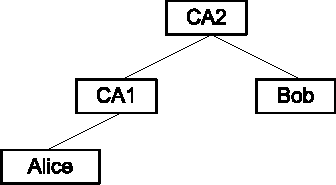
\includegraphics{Figures/pki/CA}
  \caption{Network of certificate authorities}
  \label{fig:cert authorities}
\end{figure}

Because Alice knows the public key of \emph{CA1}, she is able to
verify and willing to believe the public-key certificate for
\emph{CA2} signed by \emph{CA1}.  Such a certificate is sometimes
called a \mainindex{certificate!reverse certificate}\emph{reverse certificate},
because the signer is certifying a key for an entity higher up in the
hierarchy.  Once Alice deduces that $K_{CA2} \speaksfor \textrm{CA2}$,
she is able to verify and willing to believe the public-key
certificate for \emph{Bob} signed by \emph{CA2}.  This
certificate---in which the signer is certifying a key for an entity
lower in the hierarchy---is sometimes called a \mainindex{forward
  certificate}\emph{forward certificate}.

The following proof shows the trust assumptions made by Alice, as well as
the authorities she chooses to recognize: 

\begin{formalProof}
    1. $K_{CA1} \speaksfor \textrm{CA1}$ & trust assumption \\
    2. $K_{CA1} \says (K_{CA2} \speaksfor \textrm{CA2})$ & Key Certificate\\
    3. $K_{CA2} \says (K_{\name{Bob}} \speaksfor \textrm{Bob})$ & Key Certificate\\
    4. $\textrm{CA1} \controls (K_{CA2} \speaksfor \textrm{CA2})$ & Jurisdiction \\
    5. $\textrm{CA2} \controls (K_{\name{Bob}} \speaksfor \textrm{Bob})$ & Jurisdiction \\
    6. $\textrm{CA1} \says (K_{CA2} \speaksfor \textrm{CA2})$ & 1,2
    Derived Speaks For\\
    7. $K_{CA2} \speaksfor CA2$ & 4,6 Controls \\
    8. $\textrm{CA2} \says (K_{\name{Bob}} \speaksfor \textrm{Bob})$ &
    7, 3  Derived Speaks For \\
    9. $K_{\name{Bob}} \speaksfor \textrm{Bob}$ & 5,8  Controls
  \end{formalProof}

  The first line is Alice's belief that she knows the public key of
  \emph{CA1}. Lines two and three are the public-key certificates for
  \emph{CA2} (signed by \emph{CA1}) and \name{Bob} (signed by
  \emph{CA2}).  Lines four and five represent Alice's trust in
  \emph{CA1}'s reliability regarding certifying that $K_{CA2}$ is
  \emph{CA2}'s key, and in \emph{CA2}'s authority to say truthfully that
  $K_{\name{Bob}}$ is Bob's public key.  Lines six through nine are the
  steps necessary for Alice to deduce that $K_{\name{Bob}}$ is indeed
  Bob's public key.
\end{example}

% At this point we have developed the basic concepts of statements,
% certificates, proxies, and  jurisdiction of authority. From the
% standpoint of access control, we now have the basis for establishing who
% is making a request, under whose authority the request is being made,
% and credentials (certificates) to validate what is being said. %  In the
% % remaining sections we focus on basic access control mechanisms: tickets
% % and access-control lists.

\begin{exercise}[\appn]
  Suppose Toni sends Blake a message in the clear that is digitally
  signed as follows:
  \[(\textrm{`You're hired!''},
  \mathit{encrypt}(K^{-1}_{\name{Toni}},hash(\textrm{You're
    hired!''})))\] The above message is sent over an open channel, such
  as the Internet.  Laura intercepts the message and retransmits it to
  Blake with one crucial change: \emph{``You're hired!''} is changed to
  \emph{``You're fired!''}. Because she wants Blake to think that the
  message came from Toni, she reuses Toni's digital signature from the
  message she intercepted.

  What happens when Blake receives the message?  Is he able to detect
  the forgery or not?
\end{exercise}

\begin{exercise}[\appn]
  Use the \emph{Certificate Verification} rule to give an alternate
  proof for the situation in Example~\ref{ex:ca-chains}.
\end{exercise}

\begin{exercise}[\appn]
  This question relates to an online-purchase transaction, in which
  Zoey logs into a previously established account with her
  userid-password combination.  She then attempts to purchase an airline
  ticket, using her credit card.  In what follows, you should interpret
  $\mathit{CC}_Z$ as a principal representing a specific credit-card
  number/account.
  \begin{enumerate}
  \item Give English translations for each of the following statements,
    using notions such as \emph{authority} (or \emph{jurisdiction}),
    \emph{signatures}, \emph{sessions}, and \emph{access requests}.
%     Colloquial English is fine (and even preferred), provided your
%     translations accurately capture what's going on.

    \begin{enumerate}
    \item $\mathit{PwdServer} \controls
      (\pair{\texttt{zoey},\mathit{pwd}} \speaksfor \mathit{Zoey})$
    \item $\mathit{Visa} \controls ((\mathit{Zoey}\quoting
      \mathit{CC}_Z) \controls \mathit{buyticket})$
    \item $K_{P} \speaksfor \mathit{PwdServer}$
    \item $K_{V} \speaksfor \mathit{Visa}$
    \item $(\pair{\texttt{zoey},\mathit{pwd}}\quoting \mathit{CC}_Z)
      \says \mathit{buyticket}$
    \item $K_{P} \says (\pair{\texttt{zoey},\mathit{pwd}} \speaksfor
      \mathit{Zoey})$
    \item $K_{V} \says ((\mathit{Zoey}\quoting \mathit{CC}_Z) \controls
      \mathit{buyticket})$
    \end{enumerate}

  \item Give a formal proof that \textit{buyticket} can be deduced from
    the seven assumptions listed above.
  \end{enumerate}

\end{exercise}

\begin{exercise}[\synthesis]
  Dana has registered her public key $K_D$ with the certificate
  authority \name{CA}, whose public key is $K_\mathit{CA}$. She wishes
  to send a message $m$ to Earl, who does not know Dana and does not
  recognize the authority of \name{CA}.  Fortunately, Dana knows Earl's
  good friend Finn, who \emph{does} recognize \name{CA}'s authority.
  
  Furthermore, both Earl and Finn work at \name{Gaggle} and have
  registered their public keys ($K_E$ and $K_F$, respectively) with the
  company's certificate authority; the public key for \name{Gaggle}'s
  certificate authority is $K_G$.  (Note that both Earl and Finn have
  access to Gaggle certificates, but they have never exchanged their
  public keys with one another before.)

  Dana signs her message using her private key, and sends it to
  Finn.  She asks Finn to forward it to Earl, which Finn does as
  follows: 
  \begin{itemize}
  \item Finn uses his private key to sign Dana's signed message, and
    sends the result to Earl.
  \item Finn also gets a copy of Dana's public-key certificate, and
    signs and sends that to Earl.
  \item Finn signs a message that indicates what \name{CA}'s public
    key is, and sends that to Earl.
  \item Finally, Finn signs and sends to Earl a message stating his
    confidence in \name{CA}'s jurisdiction over Dana's public key.
  \end{itemize}

  \begin{enumerate}
  \item Express in the access-control logic the four items that Finn
    sends to Earl.
  \item Identify the additional certificates, recognitions of authority,
    and any other trust assumptions that Earl requires in order to
    deduce that the message $m$ truly came from \name{Dana}.  You
    should express each of these items in the access-control logic.
  \item Give a formal proof that $m$ can be deduced from your answers to
    parts~(a) and~(b).
  \item In your opinion, which if any of the assumptions from part~(b)
    are the most suspect?  Explain your answer.   

  \end{enumerate}
\end{exercise}
% % \chinbox{\textbf{At this point we need to say that PKI sets us up nicely
% %     to use access-control lists}}

\begin{exercise}[\synthesis]
  Two high-tech companies---\textsf{NanoTech} and
  \textsf{PicoWare}---are collaborating on a joint project called
  \textsc{Illumina}.  The project's repository and web page are housed
  at \textsf{PicoWare}'s facilities .

  When the two companies initiated this project, they established a
  special certificate authority (CA) that both companies would trust
  with respect to high-level company keys \emph{for the purposes of this
    project} only.   The public-private key pairs for the various
  entities are as follows: 

  \begin{center}
  \begin{tabular}{cl}
    $(K_{CA},K^{-1}_{CA})$ &  CA's key pair, trusted by both companies
    \\
    $(K_{N},K^{-1}_{N})$ &  \textsf{NanoTech}'s key pair, with $K_N$ registered
    with $CA$ \\
    $(K_{P},K^{-1}_{P})$ &  \textsf{PicoWare}'s key pair, with $K_P$ registered
    with $CA$ 
  \end{tabular}
  \end{center}
  This setup allows both \textsf{NanoTech} and \textsf{PicoWare} to maintain
  their existing company key infrastructures, and neither company has to
  blindly trust the other's infrastructure.  Specifically:
  \begin{itemize}
  \item \textsf{NanoTech}'s public key has been installed on all machines at
    \textsf{NanoTech}; therefore \textsf{NanoTech} machines do not need to
    fetch \textsf{NanoTech}'s 
    certificate from CA. 
  \item Likewise, \textsf{PicoWare}'s public key has been installed on all
    machines at \textsf{PicoWare}; therefore \textsf{PicoWare} machines do
    not need to fetch
    \textsf{PicoWare}'s certificate from CA.
  \item Neither company's public key has been installed on any of the
    other company's machines.  Therefore, certificates from CA are
    necessary for any secure cross-company communication.
  \item Each company certifies its own internal keys: the keys for all
    \textsf{NanoTech} employees and \textsf{NanoTech} machines are
    certified by \textsf{NanoTech}, and the keys for all
    \textsf{PicoWare} employees and \textsf{PicoWare} machines are
    certified by \textsf{PicoWare}.
  \end{itemize}

%  \textbf{Your task:} Answer the following series of questions.

  \begin{list}{(\alph{count})}{\usecounter{count}}
  \item The access-control policy for the \textsc{Illumina} project web
    page grants \textbf{both} read access (\action{\mathit{read, iwp}})
    and write access (\action{\mathit{write, iwp}}) to all members of the
    \textsc{Illumina} project.  Express this access-control policy as an
    expression in the access-control logic.  % (\emph{Note:} You do not
%     have to preface this statement with ``$\textit{ACL} \says
%     \cdots$''.)  \vspace*{1in}

  \item Stan---a \textsf{NanoTech} employee---has been issued the key pair
    $(K_S,K^{-1}_S)$.  Express Stan's public-key 
    certificate as an expression in the access-control logic.

  \item Stan has been assigned to the \textsc{Illumina} project team, and
    the group database at \textsf{PicoWare} has been updated to reflect
    this group membership.  If ever requested, the group-database server
    (GDS) can digitally sign a statement that attests to Stan's group
    membership; the group-database server's key pair is $(K_{GDS},
    K_{GDS}^{-1})$.

    Express such a certificate as an expression in the access-control
    logic.  
    \setcounter{restart}{\thecount}
  \end{list}

  Stan logs into his \textsf{NanoTech} office computer, using his
  \textsf{NanoTech}-issued smart card.  He then tries to establish an
  SSL connection to the \textsc{Illumina web page} at \textsf{PicoWare}.
  To authenticate the SSL connection, Stan's smart card uses his private
  key to cryptographically sign a response to a challenge from the
  \textsf{PicoWare} server.  The SSL connection is secured with a
  session key $K_{ssl}$.  From the point of view of the web server at
  \textsf{PicoWare}, the result of successfully establishing this SSL
  connection is the following trust assumption:
  \[ K_{ssl} \speaksfor K_{S}  \qquad (\ast) \]

  \begin{list}{(\alph{count})}%
    {\usecounter{count}\addtocounter{count}{\therestart}}%
  \item \textsf{PicoWare}'s web server receives (via SSL) Stan's request
    to read the \textsc{Illumina} web page.  Express this request as an
    expression in the access-control logic.  
  \item What are the additional certificates,
      recognition of authority, and trust assumptions regarding keys
    that are necessary for the \textsf{PicoWare} web server to determine that
    the read request should be granted? %
  \item Give a formal proof that justifies granting the request.
    Your only assumptions should be your answers to (a) through (e),
    plus the trust assumption ($\ast$).  
  \end{list}
\end{exercise}

\begin{exercise}[\synthesis]
  Some access-control decisions are made based on \emph{attributes}
  (properties such as one's age or the amount of money in your checking
  account) rather than \emph{identity}.  For example, consider what
  happens when you use a fare card like the Metro card in Washington,
  D.C.'s Metro system:
  \begin{itemize}
  \item From the standpoint of the rider, there are two resources to be
    accessed: the train at the starting destination and the exit to the
    street at the
    ending destination.

  \item The Metro card is a certificate issued by the individual Metro
    stations and possessed by the rider. Note, however, that while the
    \emph{physical card} may be the same before entering and after
    leaving the Metro station, it is \textbf{not} the same certificate:
    \begin{itemize}
    \item The information on the Metro card (particularly the amount of
      money left on the card) must be updated.
    \item The authorities that sign or vouch for the amount on the card
      are different: the turnstile used at the beginning of a rider's
      trip is different from the turnstile used at the end of the trip.
      Distinguishing the separate turnstiles (more accurately, the
      different stations) permits one to charge different amounts for
      different trips: the exit turnstile can always determine where the
      trip originated and how much to deduct from the card.
    \end{itemize}
  \end{itemize}

  To see how this works, consider a rider who wishes to travel from
  \name{Station A} to \name{Station B}, which is a trip that costs
  \$1.  Let's assume that the rider's most recent exit was at
  \name{Station C}, with a balance of \$5 on the card.
  \begin{itemize}
  \item The rider inserts the Metro card into the turnstile at
    \name{Station A}.  This card is (ultimately) interpreted as:
    \[ \name{Station C} \says (\name{balance=\$5} \wedge \name{exit=
      Station C}). \]
    Because the balance is greater than \$0, access to the train is
    granted; the card is returned to the rider saying (in effect): 
    \[ \name{Station A} \says (\name{balance=\$5} \wedge \name{entry=
      Station A}). \]
  
  \item The rider boards the train and travels to \name{Station B}.

  \item The rider inserts his or her Metro card into the turnstile at
    \name{Station B}.  Because the balance is sufficient to cover the
    cost of the trip, the turnstile returns the Metro card with an
    updated balance of \$4.
  \end{itemize}

  Assume that the turnstiles at the three stations ($A$, $B$, and $C$)
  form a private network called \name{MetroNet}.  There is a single
  certification authority \name{CA} that issues public/private key pairs
  and certifies membership in \name{MetroNet}.    The relevant
  keys are as follows:
  \begin{center}
  \begin{tabular}{cl}
    $(K_{CA},K^{-1}_{CA})$ &  CA's key pair    \\
    $(K_{A},K^{-1}_{A})$ &  \name{Station A}'s key pair    \\
    $(K_{B},K^{-1}_{B})$ &  \name{Station B}'s key pair    \\
    $(K_{C},K^{-1}_{C})$ &  \name{Station C}'s key pair 
  \end{tabular}
  \end{center}
  Digital signatures
  (based on the public and private keys distributed by the \name{CA})
  are used to provide protection against fraudulent cards.  Thus, the
  fare cards are actually digitally signed certificates.

  Use expressions in the access-control logic to answer the following
  questions regarding the certifications, credentials, and
  access-control policies needed for a rider to travel from
  \name{Station A} to \name{Station B}.
  %
  Treat attributes such as ``$\name{balance=\$5}$,''
  ``$\name{balance} > \$0$,'' and ``\name{exit= Station C}'' as simple
  propositions. Use \action{\name{enter,A}} and \action{\name{exit,B}}
  to denote entering at \name{Station A} and leaving at \name{Station
    B}, respectively.

  \begin{enumerate}
  \item  What are the necessary certificates,
      recognition of authority, and trust assumptions about keys for a
    turnstile at \name{Station B} to recognize \name{Station A} as
    belonging to \name{MetroNet}? 

  \item What are the necessary certificates,
      recognition of authority, and trust assumptions about keys for a
    turnstile at \name{Station B} to interpret an arbitrary fare card
    signed by \name{Station A}?  

  \item  What is the access policy of turnstiles at
    \name{Station A} that guard entry to trains?

  \item Assuming that a turnstile at \name{Station A} grants entry
    access to a rider, what certificate is given back to the rider as he
    or she passes through the turnstile?

  \item Assuming that a turnstile at \name{Station B} allows
    a rider to exit, what certificate is given back to the rider as he
    or she passes through the turnstile? 
  \end{enumerate}

\end{exercise}

\section{Symmetric-Key Cryptography}

\mainindex{cryptography!symmetric-key cryptography}As mentioned earlier in this
chapter, an alternative to public-key cryptography is
\mainindex{cryptography!shared key} \emph{shared-key} cryptography, also known as
\emph{symmetric-key cryptography} because the same key is used for
both encryption and decryption.  If \emph{encrypt} and \emph{decrypt}
are particular symmetric-key encryption and decryption functions, then
the following property must hold for all messages $m$ and keys $K$:
\[ \mathit{decrypt}(K,\mathit{encrypt}(K,m))  =  m. \]

\mainindex{cryptography!symmetric-key cryptography!compared with asymmetric-key
  cryptography}\mainindex{cryptography!asymmetric-key cryptography!compared with
  symmetric-key cryptography}Symmetric-key encryption
algorithms---such as the Advanced Encryption Standard (AES)
\cite{AES}---provide a significant advantage over public-key
algorithms in terms of efficiency.  They are typically three orders of
magnitude faster than public-key algorithms, because of the underlying
operations they employ (i.e., exclusive-or and bit substitutions as
opposed to modulo-$n$ exponentiation).  For this reason, it is often
preferable to encrypt large messages or files using symmetric-key
cryptography.

However, shared-key cryptography also has disadvantages that arise
from its use of a single key.  The first problem is one of planning:
Alice can send a secure message to Bob \emph{only} if they have
previously agreed upon a specific key to use.  Such an arrangement
should happen via out-of-band communication, such as during a
face-to-face meeting or some other reasonably secure means.  In
contrast, Alice can send a secure message to Bob via public-key
cryptography even if they have never communicated before, as long as
they have both published their public keys.

Another problem with shared-key cryptography is one of scale: each
principal must maintain a separate key for every other principal with
whom he or she wishes to communicate.  Thus, a collection of $n$
principals would require on the order of $n^2$ keys to support all
possible two-way conversations; public-key cryptography would require
only $2n$ keys (i.e., public and private keys for each principal). 

Finally, shared-key cryptography does not support the separation of
privacy and authenticity concerns.  For example, suppose that Alice
wishes to publish a message (i.e., allow it to be read by anyone) in a
way that provides evidence of her authorship.  We have already seen how
to accomplish this goal using public-key cryptography.  However,
symmetric-key cryptography does not support this goal directly: anyone who has
knowledge of the key to decrypt the message could forge a new message or
even claim to be the original author.

These disadvantages can be somewhat mitigated through the use of
\emph{relays} to simulate a public-key infrastructure.  We demonstrate
how later in Examples~\ref{ex:relays} and~\ref{ex:relays-auth}, but we
must first address one additional pragmatic difference between
public-key and shared-key cryptography.  A sender using public-key
cryptography can tell the recipient the relevant key to use.  For
example, if Alice sends a digitally signed message to Bob, she can also
send along her public key for his convenience.  Likewise, if she sends a
secret message to Bob using his public key, she can notify him which
public key she used; that information is useless to anyone who does not
know Bob's private key.

If Alice instead uses shared-key cryptography, then she obviously
cannot directly indicate which key Bob should use to decrypt the
message.  However, she can accomplish the same goal by sending along a
\emph{key identifier} (or \mainindex{cryptography!key hint}\emph{key hint}) that
will be meaningful only to Bob.  A \mainindex{cryptography!key identifier}key
identifier might be as simple as an index into a table of keys that is
kept on Bob's machine.  Alternatively, Bob may have a master key that
he uses to encrypt all his other keys: the key identifier for a shared
key $K$ may be the result of encrypting $K$ with that master key.  The
point here is that, when Alice and Bob set up their shared key, they
must also have exchanged their individual key identifiers associated
with that key.  However, neither needs to know \emph{how} the other
selects their key identifiers.  The following example demonstrates the
use of key identifiers.

\begin{example}\label{ex:key-hints}
  Both Richard and Janet use master keys ($K_R$ and $K_J$, respectively)
  to encrypt all their important keys.  They have recently set up a
  shared key $K_S$ that will allow them to communicate with one another
  securely.  At that time, they also exchanged key identifiers:
  \begin{itemize}
  \item Richard keeps a table of encrypted keys on his computer, and he
    likes to use the indices of this table as his key identifiers.  Richard
    adds the encrypted shared key (i.e., $\mathit{encrypt}(K_R,K_S)$) to
    this table, and gives the corresponding index (e.g., $213$) to Janet as
    the key identifier to use for this key.
  \item Janet prefers to use encrypted keys themselves as key identifiers.
    She therefore encrypts the shared key with her master key and gives
    the result to Richard as \emph{her} key identifier for the key:
    $\mathit{encrypt}(K_J,K_S)$.
  \end{itemize}

  When Janet sends a secure message to Richard using the shared key
  $K_S$, she also sends him his 
  key identifier (i.e., $213$) for the key.  Richard is able to look up the
  appropriate entry in his table (i.e., $\mathit{encrypt}(K_R,K_S)$),
  decrypt it with his master 
  key $K_R$ to obtain $K_S$, and then use $K_S$ to decrypt Janet's
  message.  

  Similarly, when Richard sends a secure message to Janet using the
  shared key $K_S$, he also includes her key identifier (i.e.,
  $\mathit{encrypt}(K_J,K_S)$).  Janet knows to decrypt this hint with
  her master key $K_J$ to obtain the key necessary to decrypt Richard's
  message.
\end{example}

As the preceding example shows, two principals may have very different
key identifiers for the same shared key.  What is important is that each
knows the other's key identifier for the shared key, so that they can
always clearly communicate which key is being used.  (In fact, two
principals may share multiple keys, using each for a different purpose.
The use of key identifiers allows them to indicate which is relevant for
the given communication.)

We adopt the notational convention\footnote{For convenience, we often
  blur the distinction between keys and key identifiers when using the
  logic.  The important point of this discussion is that key hints can
  be used both in practice and in the logic to shroud secret keys.} of
using principals' names or initials as superscripts on keys to denote
a given principal's key hint for a specific key.  For example, we use
\mainindex{cryptography!key hint!notational convention}$K_{S}^{R}$ and
$K_{S}^{J}$ to denote Richard's and Janet's key hints for the shared
key $K_S$.  We can then associate the key hints with the statements
that they make (i.e., with the messages encrypted by the keys they
hint at).  Thus, if Janet sends Richard the message $m$ encrypted with
the shared key $K_s$, we can express Richard's interpretation as
follows:
\[ K_{S}^{R} \says m. \]
If Richard trusts Janet to keep the shared key $K_S$ private, then he
should be willing to associate messages encrypted by $K_S$ with Janet.
That is, he should be willing to view the key hint
$K_{S}^{R}$ (and the key it represents) as a proxy for
Janet:
\[ K_{S}^{R} \speaksfor \name{Janet}. \]




% \begin{itemize}
% % \item Trust: Both Alice and Bob must trust each other to keep key secret.  (Is
% %   this really different from public-key case?)
% \item Planning: Alice and Bob must set up specific key prior to use
%   using out-of-band communication.  (What about data-encryption keys?)
% \item Scale: Given $n$ principals, it requires $O(n^2)$ rather than
%   $O(n)$ keys.
% \item Cannot separate privacy from authenticity: instead, must rely on
%   others to protect secrecy of key.
% \end{itemize}


The following series of examples, inspired by a discussion in
\cite{LABW}, demonstrates how a symmetric-key system can mimic a
public-key infrastructure by judicious use of key identifiers.  The
approach hinges on the use of
\mainindex{cryptography!relays}\emph{relays}, trusted agents that serve
as encryption/decryption intermediaries.  Just as any principal can
register a public-key with a certificate authority in a PKI,
\mainindex{cryptography!relays!use of to mimic PKI}the relay system
requires that any principal $Q$ be able to register with a special
trusted agent.  Furthermore, the trusted agent must know the relay's
master key, which the relay uses for creating its
\mainindex{cryptography!key hint!use with relays}key identifiers
(similar to Janet's method for key identifiers in
Example~\ref{ex:key-hints}).
% Each
% principal $P$ that 
% wishes to use the relay $R$ must share a secret key $K_P$ (plus the key
% hints  with the relay

\begin{example}\label{ex:relays}
  Quinton wishes to use symmetric encryption to send a message that
  Shelby can read and verify as being from Quinton.  Although Shelby
  and Quinton do not share a key, they have both previously
  established secret-key channels with the trusted relay $R$ by
  registering with a trusted agent $TA$.  When Quinton registered,
  $TA$ created and sent back to Quinton two items:
  \begin{enumerate}
  \item A secret key $K_q$ to be shared between Quinton and the relay
    $R$
  \item $R$'s key identifier $K_q^R = \encrypt{K_q}{K_m}$ for this key,
    which $TA$ creates by encrypting the new key $K_q$ with $R$'s master
    key $K_m$
  \end{enumerate}
  $TA$ also publishes a \mainindex{certificate!secret-key
    certificate}\emph{secret-key certificate} for Quinton that
  contains two components
  \symindex{$<\negthickspace\negthickspace<m_1,m_2,\ldots,
    m_k>\negthickspace\negthickspace>$: concatenation}(we introduce the
  notation \cat{m_1,m_2,\ldots, m_k} to denote the concatenation of
  the $k$ items $m_1$ through $m_k$):
  \[ \encrypt{\cat{K_q^Q,K_q^R,\name{Quinton}}}{K_{ta}}, \quad
  K_{ta}^R. \]
  The first item associates the pair $(K_q^Q, K_q^R)$ of key identifiers
  with Quinton; this item is signed by $TA$ using the key $K_{ta}$ that
  it shares with the relay.  The second item is the relay's key hint for
  the shared key $K_{ta}$, so that anyone who wishes to read the
  certificate can direct the relay which key to use for decryption.
%   \item Quinton's \emph{shared-key certificate}, signed with the key
%     that $TA$ shares with $R$ ($K_{ta}$) and combined with the
%     appropriate key hint for this key ($K_{ta}^R$):
%     \[ \encrypt{\cat{K_q^Q,K_q^R,\name{Quinton}}}{K_{ta}}, \qquad
%     K_{ta}^R \]
  Unlike a public-key certificate, the shared-key certificate
  is not readable by just anybody: only a principal that knows the
  secret key $K_{ta}$ (such as $TA$ and the relay) can read it.

%   $TA$ gave both the key and
%   $R$'s key identifier to Quinton, who is able to construct his own key
%   identifier $K_q^Q$ for the key.  In a similar fashion, Shelby shares a
%   key $K_s$ with the relay and knows the relay's key identifer $K_s^R$
%   for that key.

  Quinton encrypts his message $m$ with the key $K_q$, sending both the
  encrypted message and the key hint $K_q^R$ to Shelby:
  \[ \encrypt{m}{K_q}, \quad K_q^R. \] Shelby cannot decrypt the message
  directly, because she does not know the shared key that $K_q^R$
  identifies.  However, 
  because Shelby also registered with $TA$, she shares a secret key
  $K_s$ with the relay and knows the relay's key hint $K_s^R$ for that
  key.  She therefore forwards these items on to the relay $R$, along
  with the key-identifier pair $(K_s^S,K_s^R)$.  In effect, Shelby is
  requesting a decryption of the encryption message and telling the
  relay how to return the answer.  (Shelby can also forward on Quinton's
  shared-key certificate for decryption, if she wishes to authenticate
  the message.  We leave this possibility for Example~\ref{ex:relays-auth}.) 

  The relay applies its master key $K_m$ to the key hint $K_q^R$ to
  obtain the key $K_q$:
  \[ \mathit{decrypt}(K_m, K_q^R) = \mathit{decrypt}(K_m,
  \encrypt{K_q}{K_m}) = K_q. \] 
  With this key, the relay can decrypt the message \encrypt{m}{K_q} to
  obtain the original message $m$:
  \[ \mathit{decrypt}(K_q, \encrypt{m}{K_q}) = m . \] 
  The relay then repackages this message for Shelby by encrypting $m$
  with the shared key $K_s = \mathit{decrypt}(K_m, K_s^R)$, sending back
  the newly encrypted version as well as the key hint $K_s^S$:
  \[ \encrypt{m}{K_s}, \quad K_s^S. \]

  Upon receiving this package, Shelby uses the key hint $K_s^S$ to
  identify the correct key ($K_s$) to use to decrypt the message:
  \[ \mathit{decrypt}(K_s, \encrypt{m}{K_s}) = m.  \]
  As a result of this process, Shelby interprets this message as follows:
  \[ K_s^S \says K_q^R \says m. \]
  That is, the key identifier $K_s^S$ is claiming that the key hint
  $K_q^R$ was used to send the message $m$.  If Shelby trusts the relay
  to keep the key $K_s$ secret (i.e., if she believes that $K_s^S
  \speaksfor R$) and to accurately translate messages (i.e., $R
  \controls K_q^R \says m$), then she will deduce that $m$ was the
  original intended message she received (i.e., $K_q^R \says m$).
\end{example}

The previous example demonstrated how secret-key cryptography can be
used to exchange messages between principals who have not previously
established a shared secret key.  However, the example as it stands does
not address authentication concerns: neither the relay nor Shelby are
able to associate the key identifier $K_q^R$ with Quinton at the end of
the process described.  To do so, they must also make use of Quinton's
secret-key certificate as demonstrated in the next example. 


\begin{example}\label{ex:relays-auth}
%   Recall from the previous example that the trusted authority $TA$ knows
%   the relay's master key and can therefore always calculate the relay's
%   key identifier for any given secret key.  When Quinton initially
%   registers with $TA$, $TA$ publishes a secret-key certificate containing the
%   following two components:
%   \[ \encrypt{\cat{K_q^Q,K_q^R,\mathit{Quinton}}}{K_{ta}}, \quad
%   K_{ta}^R. \]
%   The first item associates the pair $(K_q^Q, K_q^R)$ of key identifiers
%   with Quinton; this item is signed by $TA$ using the key $K_{ta}$ that
%   it shares with the relay.  The second item is the relay's key hint for
%   the shared key $K_{ta}$, so that anyone who wishes to read the
%   certificate can direct the relay which key to use for decryption.
  By the end of Example~\ref{ex:relays}, Shelby had deduced that $K_q^R
  \says m$.  If she wishes to authenticate Quinton as the message's author
  (i.e., to associate the key hint $K_q^R$ with Quinton), then she
  forwards Quinton's secret-key certificate to the relay along with her
  key-hint pair $(K_s^S,K_s^R)$.  As with the original message, the
  relay can decrypt the certificate, 
  which can be expressed in the logic as follows:
  \[ K_{ta}^R \says ((K_q^Q, K_q^R) \speaksfor \name{Quinton}). \]
  That is, the key hint $K_{ta}^R$ claims that the key-hint pair
  $(K_q^Q, K_q^R)$ is associated with Quinton.  If the relay trusts that
  the key hint $K_{ta}^R$ (i.e., the key $K_{ta}$) represents $TA$ and
  that $TA$ has jurisdiction over which keys represent which principals,
  then it will be able to associate the key hint $K_q^R$ with
  $\name{Quinton}$.

  At this point, the relay must create for Shelby a new certificate that
  associates the key hint $K_q^R$ with Quinton.  The relay sends the
  following items to Shelby:
  \[ \encrypt{\cat{K_q^R,\name{Quinton}}}{K_s}, \quad K_s^S. \] 
  As before, Shelby can decrypt the message to interpret the certificate
  as follows:
  \[ K_s^S \says (K_q^R \speaksfor \name{Quinton}). \]
\end{example}

As a final twist on this scenario, suppose that Shelby wishes to
exchange a series of messages with Quinton.  She may wish to set up
an authenticated channel between herself and Quinton, so that they can
exchange messages directly without having to use the relay for continual
translations.   As the following example demonstrates, Shelby can enlist
the relay's help to set up such a channel. 

\begin{example}\label{ex:relays-auth-channel}
  To set up an authenticated channel with Quinton, Shelby proceeds in
  the same way as at the beginning of Example~\ref{ex:relays-auth}.  
  She
  forwards Quinton's secret-key certificate to the relay along with her
  key-hint pair $(K_s^S,K_s^R)$.  The relay decrypts this certificate
  and interprets it as before:
  \[ K_{ta}^R \says ((K_q^Q, K_q^R) \speaksfor \name{Quinton}). \]
%   That is, the key hint $K_{ta}^R$ claims that the key-hint pair
%   $(K_q^Q, K_q^R)$ is associated with Quinton.  If the relay trusts that
%   the key hint $K_{ta}^R$ (i.e., the key $K_{ta}$) represents $TA$ and
%   that $TA$ has jurisdiction over which keys represent which principals,
%   then it will be able to associate the key hint $K_q^R$ with
%   $\name{Quinton}$.

  The relay now creates a new channel for direct
  communication between Quinton and Shelby.  Specifically, the relay
  creates a new key $K$ and creates key identifiers for Quinton and
  Shelby by encrypting it with their individual keys:
  \[ K^Q = \encrypt{K}{K_q}, \qquad K^S = \encrypt{K}{K_s}. \]
  The relay then creates a new certificate for Shelby that associates
  this new key-hint pair $(K^Q,K^S)$ with Quinton:
  \[ \encrypt{\cat{K^Q,K^S,\name{Quinton}}}{K_s}, \quad
  K_s^S. \]
  Shelby can interpret this certificate as follows:
  \[ K_s^S \says ((K^Q, K^S) \speaksfor \name{Quinton}). \] 
  (If Quinton wishes to also authenticate Shelby, then the relay will
  need to obtain Shelby's original secret-key certificate and then
  generate a new one for Quinton to use in a similar fashion.)
\end{example}

\begin{exercise}[\eval]Consider the certificate that Shelby receives at
  the end of   Example~\ref{ex:relays-auth}.
  \begin{enumerate}
  \item What additional trust assumptions must Shelby make in order to
    identify Quinton as the sender of the original message from
    Example~\ref{ex:relays}?
  \item Another possible interpretation in the logic of that certificate
    is as follows:
    \[ K_s^S \says (K_s^S \quoting K_q^R \speaksfor \name{Quinton}). \]
    Given this interpretation, what additional trust assumptions must
    Shelby make in order to identify Quinton as the sender of the
    original message from Example~\ref{ex:relays}?
  \item Briefly describe the advantages and disadvantages of the two
    interpretations, and identify the situations where each might be
    more appropriate.
  \end{enumerate}


\end{exercise}

\begin{exercise}[\appn]
  What additional trust assumptions must Shelby make to associate the
  new key $K$ (or its associated key-hint pair) with Quinton in
  Example~\ref{ex:relays-auth-channel}? 
\end{exercise}

\begin{exercise}[\synthesis]
  Suppose that two-way authentication is necessary in
  Example~\ref{ex:relays-auth-channel} (i.e., Quinton also wishes to
  authenticate Shelby).
  \begin{enumerate}
  \item What messages need to be sent between Quinton and the relay?
  \item Express in the access-control logic how these messages are
    interpreted, along with the trust assumptions necessary for the
    protocol to succeed.
  \end{enumerate}
\end{exercise}



% \begin{exercise}[\synthesis]
%   Kerberos is a protocol that provides secure authentication for
%   principals on an insecure network, using symmetric (i.e., shared-key)
%   encryption.  In a nutshell, here's how Kerberos works:
%   \begin{description}
%   \item[(1)] A user Claude logs into his workstation, and enters his
%     password.  A program running on the workstation (i.e., the
%     \emph{client}) does two things: (1) it sends unencrypted the user's
%     name to the \emph{Authentication Server (AS)}, and (2) it runs a
%     predetermined one-way hash function on Claude's password to
%     create the \emph{client's secret key} ($K_{C}$).  (Note: By
%     generating this key fresh, the workstation does not need to store it
%     when Claude is not logged in.  However, the same key will have been
%     previously stored by the AS.)
%   \item[(2)] The AS looks Claude's username up in its database, to ensure that
%     Claude is an authorized user.  Along with the listing for Claude is Claude's
%     secret key $K_C$.  The AS sends two items back to the client:
%     \begin{itemize}
%     \item A newly generated \emph{session key} $K_{c,tgs}$ through which
%       the client can communicate with the \emph{ticket-granting server
%         (TGS)}; this key is encrypted with the client's secret key $K_C$.
%     \item A ticket that associates the session key $K_{c,tgs}$ with the
%       client (including the client's id and network address, a ticket validity
%       period, etc); this ticket is encrypted with the key $K_{TGS}$,
%       which is shared by AS and TGS.
%     \end{itemize}
%   \item[(3)] Now, when Claude wants to (say) print a file, he needs to 
%     authenticate to the \emph{Print Server (PS)}; to do so, he must 
%     first get a ticket from the TGS.  Therefore, the client on Claude's
%     behalf sends the following three items to TGS:
%     \begin{itemize}
%     \item The name of the server it wishes to authenticate to (in this
%       case, \name{PS}) 
%     \item The ticket that AS had sent to the client on the previous step
%       (i.e., the one encrypted with $K_{TGS}$)
%     \item An \emph{authenticator}, which is a message that contains the
%       client's id and is encrypted with the session key $K_{c,tgs}$
%     \end{itemize}
%   \item[(4)] The TGS uses its secret key $K_{TGS}$ to decrypt the ticket,
%     after which it can use the session key $K_{c,tgs}$ to decrypt the
%     authenticator and verify that the client making the request is the
%     one authorized by AS to do so.  Assuming everything checks out, the
%     TGS sends a new ticket to the client that can be used to request
%     services from the Print Server.
%   \end{description}
%   The Kerberos protocol continues for a few more steps, but this
%   question concerns only the decision made in Stage~4 described above.
% %   The three items that the client sends to the TGS in Stage~3 can be
% %   interpreted as statements in the logic as follows:
% %   \begin{itemize}
% %   \item The name of the server it wishes to authenticate to (in this
% %     case, \name{PS}) 
% %     \[ \name{client@address} \says \action{\name{get ticket,PS}} \]
% %   \item The ticket that AS had sent to the client on the previous step
% %     (i.e., the one encrypted with $K_{TGS}$)

% % %    \[ K_{TGS} \says (K_{c,tgs} \speaksfor \name{client@address}) \]
% %     \[ K_{TGS} \says (K_{c,tgs} \controls (\name{client@address}
% %     \controls \action{\name{get ticket, PS}}))  \]
% %   \item An \emph{authenticator}, which is a message that contains the
% %     client's id and is encrypted with the session key $K_{c,tgs}$

% %     \[ K_{c,tgs} \says (\name{client@address} \controls
% %     \action{\name{get ticket,PS}}) \] 
% %   \end{itemize}
% %   \textsc{Important note:} \emph{In lecture, we discussed how pairs of
% %     key identifiers can be used to name shared-key encryption channels.
% %     To keep the notation simple in this question, I am using the shared
% %     keys directly to name the channels.}


%   Consider an analysis of this situation from the point of view
%   of the \textbf{ticket-granting server (TGS)}, as it determines whether
%   or not to grant the requested ticket.
%   Specifically, the three items that the client sends to the TGS in
%   Stage~3 can be interpreted as statements in the logic as follows:
%   \begin{itemize}
%   \item The name of the server it wishes to authenticate to (in this
%     case, \name{PS}) 
%     \[ \name{client@address} \says \action{\name{get ticket,PS}} \]
%   \item The ticket that AS had sent to the client on the previous step
%     (i.e., the one encrypted with $K_{TGS}$)

% %    \[ K_{TGS} \says (K_{c,tgs} \speaksfor \name{client@address}) \]
%     \[ K_{TGS} \says (K_{c,tgs} \controls (\name{client@address}
%     \controls \action{\name{get ticket, PS}}))  \]
%   \item An \emph{authenticator}, which is a message that contains the
%     client's id and is encrypted with the session key $K_{c,tgs}$

%     \[ K_{c,tgs} \says (\name{client@address} \controls
%     \action{\name{get ticket,PS}}) \] 
%   \end{itemize}
%   \textsc{Important note:} \emph{In lecture, we discussed how pairs of
%     key identifiers can be used to name shared-key encryption channels.
%     To keep the notation simple in this question, I am using the shared
%     keys directly to name the channels.}

%   \begin{enumerate}
%   \item The TGS must recognize the jurisdiction of one or
%     more authorities, and make one or more additional trust assumptions,
%     in order to grant the ticket: what are they?  Express your answers
%     as statements in the access-control logic. 
%   \item Give a formal proof that the request can be granted,
%     using as your only assumptions the three statements given above
%     plus your answers to Part~(2).
%   \end{enumerate}

% \end{exercise}


\section{Summary}

We have already seen that authentication---that is, identifying the
originator of a request---is critical to sound access control.  In the
digital world, authentication is made more difficult by the physical
absence of the requesting principal: a request arrives as a sequence of
bits, with only hints of its origin.  

In this chapter, we saw how public-key infrastructures support digital
authentication through the use of public and private keys, digital
signatures, public-key certificates, and certificate authorities.  A PKI
supports integrity, privacy, and authentication by providing the means
to associate specific keys---and, subsequently, specific
statements---with specific principals.  We explored how to express and
reason about the fundamental concepts of PKI in the access-control
logic. We also discussed the main differences between symmetric
and asymmetric cryptography.

The learning outcomes associated with this chapter appear in
Figure~\ref{fig:outcomes-chap6}.

\begin{figure}[tb]
  \centering
After completing this chapter, you should be able to achieve the following
learning outcomes at several levels of knowledge:
\begin{description}
\item[Comprehension] \
  \begin{itemize}
  \item Describe the characteristics of private-key and secret-key
    cryptographic systems.
  \item Describe basic principles of trust topologies and networks of
    certification authorities.
  \end{itemize}
\item[Application] \
  \begin{itemize}
  \item When given protocol descriptions and trust hierarchies, you
    should be able to use the access-control logic to describe the
    protocol and trust relationships.
  \item When given a trust topology, you should be able to determine the
    necessary certificates for establishing trust in a key.
  \end{itemize}
\item[Analysis] \
  \begin{itemize}
  \item When given a set of certificates, you should be able to formally
    derive whether a key is associated with a particular principal.
  \end{itemize}
\item[Synthesis] \
  \begin{itemize}
  \item When given a description of a trust topology, you should be able
    to create a formal description of the certificates and trust
    relationships for the certification authorities.
  \end{itemize}
\end{description}
  
  \caption{Learning outcomes for Chapter~6}
  \label{fig:outcomes-chap6}
\end{figure}

\section{Further Reading}
The \emph{Handbook of Applied Cryptography} \cite{Handbook} is a very
mathematical and authoritative reference for cryptographic algorithms,
hash algorithms, digital signatures, and cryptographic protocols.
William Stallings' book \emph{Cryptography and Network Security
  Principles and Practices} \cite{Stallings} is a less comprehensive but
more accessible reference.

% ---- this points LaTeX to book.tex ----
%%% Local Variables:
%%% TeX-master: "book"
%%% End:

%  LocalWords:  PKI RSA cryptosystem checksum AES dek plaintext Zoey
%  LocalWords:  GoodBooks TrueSignatures online userid PwdServer zoey
%  LocalWords:  pwd buyticket NanoTech PicoWare Illumina other's iwp
%  LocalWords:  GDS SSL ssl one's MetroNet indices getMessage deciphS
%  LocalWords:  Accessor datatype msg SymKey symMsg sym num deciphP
%  LocalWords:  pKey asymMsg princ pubK privK signVerify signVerifyOK
%  LocalWords:  Stallings
